%definira klasu dokumenta 
\documentclass[12pt]{report} 

%prostor izmedu naredbi \documentclass i \begin{document} se zove uvod. U njemu se nalaze naredbe koje se odnose na cijeli dokument

%osnovni LaTex ne može riješiti sve probleme, pa se koriste različiti paketi koji olakšavaju izradu željenog dokumenta
\usepackage[croatian]{babel} 
\usepackage{amssymb}
\usepackage{amsmath}
\usepackage{txfonts}
\usepackage{mathdots}
\usepackage{titlesec}
\usepackage{array}
\usepackage{lastpage}
\usepackage{etoolbox}
\usepackage{longtable, tabu}
\usepackage{color, colortbl}
\usepackage{adjustbox}
\usepackage{geometry}
\usepackage[classicReIm]{kpfonts}
\usepackage{hyperref}
\usepackage{fancyhdr}

\usepackage{float}
\usepackage{setspace}
\restylefloat{table}


\patchcmd{\chapter}{\thispagestyle{plain}}{\thispagestyle{fancy}}{}{} %redefiniranje stila stranice u paketu fancyhdr

%oblik naslova poglavlja
\titleformat{\chapter}{\normalfont\huge\bfseries}{\thechapter.}{20pt}{\Huge}
\titlespacing{\chapter}{0pt}{0pt}{40pt}


\linespread{1.3} %razmak između redaka

\geometry{a4paper, left=1in, top=1in,}  %oblik stranice

\hypersetup{ colorlinks, citecolor=black, filecolor=black, linkcolor=black,	urlcolor=black }   %izgled poveznice


%prored smanjen između redaka u nabrajanjima i popisima
\newenvironment{packed_enum}{
	\begin{enumerate}
		\setlength{\itemsep}{0pt}
		\setlength{\parskip}{0pt}
		\setlength{\parsep}{0pt}
	}{\end{enumerate}}

\newenvironment{packed_item}{
	\begin{itemize}
		\setlength{\itemsep}{0pt}
		\setlength{\parskip}{0pt}
		\setlength{\parsep}{0pt}
	}{\end{itemize}}


%boja za privatni i udaljeni kljuc u tablicama
\definecolor{LightBlue}{rgb}{0.9,0.9,1}
\definecolor{LightGreen}{rgb}{0.9,1,0.9}


%podesavanje zaglavlja i podnožja

\pagestyle{fancy}
\lhead{Programsko inženjerstvo}
\rhead{$<$Humanitarni šetači pasa$>$}
\lfoot{OneClick}
\cfoot{stranica \thepage/\pageref{LastPage}}
\rfoot{\today}
\renewcommand{\headrulewidth}{0.2pt}
\renewcommand{\footrulewidth}{0.2pt}


\begin{document} 
	
	
	
	\begin{titlepage}
		\begin{center}
			\vspace*{\stretch{1.0}} %u kombinaciji s ostalim \vspace naredbama definira razmak između redaka teksta
			\LARGE Programsko inženjerstvo\\
			\large Ak. god. 2020./2021.\\
			
			\vspace*{\stretch{3.0}}
			
			\huge Humanitarni šetači pasa\\
			\Large Dokumentacija, Rev. 1
			
			\vspace*{\stretch{12.0}}
			\normalsize
			Grupa: \textit{OneClick}\\
			Voditelj: \textit{Benjamin Horvat}\\
			
			
			\vspace*{\stretch{1.0}}
			Datum predaje: \textit{13. 11. 2020.}\\
	
			\vspace*{\stretch{4.0}}
			
			Nastavnik: \textit{Doria Bukić}\\
		
		\end{center}

	
	\end{titlepage}

	
	\tableofcontents

	\chapter{Dnevnik promjena dokumentacije}
		
				
		
		\begin{longtabu} to \textwidth {|X[2, l]|X[13, l]|X[3, l]|X[3, l]|}
			\hline \multicolumn{1}{|l|}{\textbf{Rev.}}	& \multicolumn{1}{l|}{\textbf{Opis promjene/dodatka}} & \multicolumn{1}{|l|}{\textbf{Autori}} & \multicolumn{1}{l|}{\textbf{Datum}} \\[3pt] \hline
			\endfirsthead
			
			\hline \multicolumn{1}{|l|}{\textbf{Rev.}}	& \multicolumn{1}{l|}{\textbf{Opis promjene/dodatka}} & \multicolumn{1}{|l|}{\textbf{Autori}} & \multicolumn{1}{l|}{\textbf{Datum}} \\[3pt] \hline
			\endhead
			
			\hline 
			\endlastfoot
			
			0.1 & Promijenjena naslovna stranica.	& Horvat & 15.10.2020. 		\\[3pt] \hline 
			0.2	& Upisani dionici. & Mužević & 22.10.2020. 	\\[3pt] \hline 
			0.3 & Upisani \textit{Use Case}vi: 1-4, 6, 6.1, 7 i 7.1. \newline Upisani aktori i njihovi funkcionalni zahtjevi. & Čovran \newline Doljanin \newline Mužević & 28.10.2020. \\[3pt] \hline 
			0.4 & Upisani \textit{Use Case}vi: 5, 8, 9, 10. & Doljanin & 02.11.2020. \\[3pt] \hline 
			0.5 & UML i sekvencijski dijagrami.\newline Baza podataka i ER dijagram. \newline UC10 promijenjen u UC10.1 te dodan novi UC10. & Horvat & 06.11.2020. \\[3pt] \hline 
			0.6 & Opis projektnog zadatka & Zekić & 10.11.2020. \\[3pt] \hline 
			0.7 & Dijagrami razreda. \newline Izbrisane smjernice. \newline Predgovor za arhitekturu sustava. \newline Popravak UC1.  & Horvat, Mirković, Doljanin & 11.11.2020. \\[3pt] \hline 
			0.8 & Upis broja sati. \newline Popravak dokumentacije. \newline Upisan dnevnik sastajanja. & Zekić, Mirković, Doljanin, Čovran, Rodek & 12.11.2020. \\[3pt] \hline 
			\textbf{1.0} & Ažurirani dijagrami razreda. \newline Zadnji popravci.  & Horvat & 13.11.2020. \\[3pt] \hline 
			&  &  & \\[3pt] \hline
			
			
		\end{longtabu}
	
	
	\chapter{Opis projektnog zadatka}
		
		\section{Opis problema i cilj projekta}
		U današnjem svijetu nezbrinute i napuštene životinje nisu stran pojam. Procijenjeno je kako u Hrvatskoj gotovo 10.000 životinja nema svoj dom. Nasreću, postoje udruge i ustanove koje napuštenim životinjama pružaju osnovnu njegu i toplinu. Te udruge i skloništa spašavaju ranjene i nezbrinute životinje, no često su im kapaciteti popunjeni, a radnici imaju previše posla. S motivacijom da se s jedne strane pomogne radnicima pri brizi za životinje, a s druge strane potakne građane na angažiranost i udomljavanje životinja, nastala je ideja za aplikaciju „Humanitarni šetači pasa“. Glavni je zadatak aplikacije povezati udruge za životinje s građanima koji imaju želju i vrijeme za šetanje pasa te time povećati izglede udomljavanja pasa i psihološkog efekta dobrobiti socijalizacije za psa i za čovjeka.
		
		
		\section{Funkcionalnosti}
		Pokretanjem aplikacije otvara se naslovna stranica na kojoj je prikazano zaglavlje te popis svih registriranih udruga.
		\newline
		Neregistrirani korisnik ima mogućnost pregleda popisa te pretraživanja udruga po nazivu ili lokaciji. Odabirom pojedine udruge otvaraju se detalji njezina profila. U sklopu profila udruge korisnik može dobiti informacije o psima (slike i opisi, raspoloživost za šetnju u određenom vremenskom periodu (datum i vrijeme) te jesu li psi predodređeni za skupne ili za individualne šetnje). Dodatno, prilikom pregleda profila korisniku je dostupna i rang lista registriranih šetača poredanih s obzirom na broj šetnji, broj pasa te duljinu šetnje koju su odradili u posljednjih mjesec dana. Također, dostupne su mu informacije na kojoj se lokaciji nalazi udruga, statistika o šetnjama svih pasa te mogućnost da se prijavi za šetnju pasa. Ako se korisnik odluči na potonju opciju, ima mogućnost prijave u sustav ili registracije ukoliko još nema račun.
		\newline
		Prilikom registracije korisnik bira želi li se prijaviti kao građanin ili kao udruga.
		\newline
		\newline
		Za registraciju građanina potrebno je unijeti:
		\begin{itemize}
			\item korisničko ime
			\item e-mail
			\item ime i prezime
			\item lozinka
			\item broj mobitela
		\end{itemize}
		
		\noindent
		Za registraciju udruge potrebno je unijeti:
	
		\begin{itemize}
			\item naziv
			\item OIB udruge
			\item korisničko ime
			\item adresu
			\item mjesto
			\item e-mail
			\item lozinku
		\end{itemize}
		
		\noindent
		Registracijom u sustav kao građanin, korisniku se otvara mogućnost prijave za šetnju, pregledavanja osobnih podataka, vlastite statistike šetnji te pregledavanja i preuzimanja vlastitog rasporeda u PDF formatu. On svoju statistiku šetnji može označiti javnom kako bi ona dospjela na rang listu na javnoj stranici.
		\newline
		Udruga registracijom, osim mogućnosti prijave u sustav te pregleda vlastitih osobnih podataka, dobiva i mogućnost mijenjanja profila životinja.
		
		\eject
	
	\chapter{Specifikacija programske potpore}
		
	\section{Funkcionalni zahtjevi}
			
			
			
			\noindent \textbf{Dionici:}
			
			\begin{packed_enum}
				
				\item Administrator
				\item Građanin
				\item Javni posjetitelj
				\item Razvojni tim
				\item Udruga za životinje
				\item Životinja 
				
			\end{packed_enum}
			
			\noindent \textbf{Aktori i njihovi funkcionalni zahtjevi:}
			
			
			\begin{packed_enum}
				\item  \underbar{Neregistrirani/neprijavljeni korisnik (inicijator) može:}
				
				\begin{packed_enum}
					
					\item Pristupiti naslovnoj stranici na kojoj može pregledati sve udruge
					\item Pristupiti detaljima profila udruge za životinje
					\begin{packed_enum}
						
						\item Dobiti uvid u profile pasa
						\item Dobiti uvid u statistike
						
					\end{packed_enum}
					\item Pristupiti rang listi
					\item Imati mogućnost registracije kao građanin ili udruga za životinje
					
				\end{packed_enum}
			
				\item  \underbar{Građani (inicijator) mogu:}
				
				\begin{packed_enum}
					
					\item Imati sve mogućnosti neprijavljenog/neregistiranog korisnika
					\item Prijaviti se u vlastiti profil
					\item Pregledati svoj raspored šetnji i svoje statistike šetnji
					\item Učiniti svoje statistike šetnji javnima
					\item Odabrati psa i željeni termin šetnje
					\item Preuzeti svoj raspored šetnji kao PDF 
					\item Mijenjati podatake o svom profilu
					
				\end{packed_enum}
			
				\item  \underbar{Udruge za životinje (inicijator) mogu:}
				
				\begin{packed_enum}
					
					\item Prijaviti se u vlastiti profil
					\item Mijenjati podatake o svom profilu
					\item Pristupiti naslovnoj stranici na kojoj može pregledati sve udruge
					\item Pristupiti profilima životinja i udruga za životinje
					
				\end{packed_enum}
			
				\item  \underbar{Administrator (inicijator) može:}
				
				\begin{packed_enum}
					
					\item Upravljati profilima građana, udruga i životinja
					\item Upravljati šetnjama
					
				\end{packed_enum}
			
				\item \underbar{Baza podataka (sudionik)}
				
					\begin{packed_enum}
						
						\item Dohvaćati podatke
						\item Pohranjivati podatke
						
					\end{packed_enum}
					
			
			\end{packed_enum}
			
			\eject 
			
			
				
			\subsection{Obrasci uporabe}
				
	
					
					\noindent \underbar{\textbf{UC1 - Registracija u sustav}}
					\begin{packed_item}
	
						\item \textbf{Glavni sudionik: } Javni posjetitelj
						\item  \textbf{Cilj:} Registracija u sustav kao građanin ili udruga za životinje
						\item  \textbf{Sudionici:} Baza podataka
						\item  \textbf{Preduvjet:} Korisničko ime i e-mail ne smiju biti već iskorišteni
						\item  \textbf{Opis osnovnog tijeka registracije udruge:}

						\item[] \begin{packed_enum}
							
							\item Odabir registracije udruge
							\item Unos korisničkog imena
							\item Unos e-mail adrese
							\item Unos lozinke
							\item Unos naziva udruge
							\item Unos broja telefona udruge
							\item Unos OIB-a udruge
							\item Unos adrese udruge
							\item Kliknuti gumb "Registracija"
							
							\end{packed_enum}
						
						\item  \textbf{Opis osnovnog tijeka registracije građanina:}
						
						\item[] \begin{packed_enum}
							
							\item Odabir registracije građanina
							\item Unos korisničkog imena
							\item Unos lozinke
							\item Unos imena
							\item Unos prezimena
							\item Unos e-mail adrese
							\item Unos broja telefona
							\item Kliknuti gumb "Registracija"
							
						\end{packed_enum}
					
						\item  \textbf{Opis mogućih odstupanja:}
					
						\item[] \begin{packed_item}
	
							\item[1.a] Korisničko ime već postoji u sustavu
							\item[] \begin{packed_enum}
								
								\item Sustav obavještava korisnika da unese drugo korinsičko ime
								\item Korisnik mijenja potrebne podatke te završava unos ili odustaje od registracije
								
								
								\end{packed_enum}
							\item[2.a] E-mail već postoji u sustavu
							\item[] \begin{packed_enum}
								
								\item Sustav obavještava korisnika da unese drugi e-mail
								\item Korisnik mijenja potrebne podatke te završava unos ili odustaje od registracije
								\end{packed_enum}
							
							
							\end{packed_item}
					\end{packed_item}
				
				\noindent \underbar{\textbf{UC2 - Prijava u sustav}}
					\begin{packed_item}
						
						\item \textbf{Glavni sudionik: } Građanin ili udruga
						\item  \textbf{Cilj:} Prijava u sustav kao građanin ili udruga
						\item  \textbf{Sudionici:} Baza podataka
						\item  \textbf{Preduvjet:} Građanin ili udruga moraju biti registrirani u sustav
						\item  \textbf{Opis osnovnog tijeka:}
						
						\item[] \begin{packed_enum}
							
							\item Unos korisničkog imena
							\item Unos lozinke
							\item Kliknuti gumb "Prijava"
						\end{packed_enum}
						
						\item  \textbf{Opis mogućih odstupanja:}
						
						\item[] \begin{packed_item}
							
							\item[1.a] Korisničko ime ne postoji u sustavu
							\item[] \begin{packed_enum}
								
								\item Sustav obavještava korisnika da je uneseno nepostojeće 
								korisničko ime
								\item Korisnik mijenja potrebne podatke te završava unos ili odustaje 
								od prijave
								
								
								
							\end{packed_enum}
							\item[2.a] Korisnik je unio krivu lozinku za navedeno korisničko ime
							\item[] \begin{packed_enum}
								
								\item Sustav obavještava korisnika da unese ispravnu lozinku
								\item Korisnik unosi ispravnu lozinku ili odustaje 
								od prijave
								
							\end{packed_enum}	
							
						\end{packed_item}
					\end{packed_item}
					
				\noindent \underbar{\textbf{UC3 - Pregled naslovne stranice}}
					\begin{packed_item}
						
						\item \textbf{Glavni sudionik: } Korisnik
						\item  \textbf{Cilj:} Pregled liste udruga
						\item  \textbf{Sudionici:} Baza podataka
						\item  \textbf{Preduvjet:} Pristup aplikaciji
						\item  \textbf{Opis osnovnog tijeka:} 
						
						\item[] \begin{packed_enum}
							
							\item Otvaranje aplikacije ili klik na gumb “Početna stranica”
							\item Pregled dostupnih podataka
						\end{packed_enum}
						
					\end{packed_item}
					
					\noindent \underbar{\textbf{UC3.1 - Pregled detalja udruga}}
					\begin{packed_item}
						
						\item \textbf{Glavni sudionik: } Korisnik
						\item  \textbf{Cilj:} Prikaz detalja udruga
						\item  \textbf{Sudionici:} Baza podataka
						\item  \textbf{Preduvjet:} -
						\item  \textbf{Opis osnovnog tijeka:} 
						
						\item[] \begin{packed_enum}
							
							\item Odabir željene udruge na naslovnoj stranici
							\item Prikaz podataka udruge
							\end{packed_enum}
						
					\end{packed_item}
					
				\noindent \underbar{\textbf{UC4 - Pretraživanje udruga}}
					\begin{packed_item}
						
						\item \textbf{Glavni sudionik: } Korisnik
						\item  \textbf{Cilj:} Pronaći udrugu preko upisa imena ili lokacije
						\item  \textbf{Sudionici:} Baza podataka
						\item  \textbf{Preduvjet:} -
						\item  \textbf{Opis osnovnog tijeka:} 
						
						\item[] \begin{packed_enum}
							
							\item Odabrati gumb "Pretraživanje" i upisati u polje za pretraživanje
							\item Odabrati željenu udrugu
							\end{packed_enum}
						
					\end{packed_item}
				
					\noindent \underbar{\textbf{UC5 - Prijava šetnje}}
					\begin{packed_item}
						
						\item \textbf{Glavni sudionik: } Građanin
						\item  \textbf{Cilj:} Prijaviti šetnju sa željenom životinjom i željenim terminom
						\item  \textbf{Sudionici:} Životinje, Baza podataka
						\item  \textbf{Preduvjet:} Prijavljen u sustav
						\item  \textbf{Opis osnovnog tijeka:}
						
						\item[] \begin{packed_enum}
							
							\item Odabire se željeni termin i duljina šetnju
							\item Odaberu se svi željeni psi za šetnju koji su slobodni u odabranom terminu te koji odgovaraju vrsti šetnje
							\item Odabire se opcija “Prijavi šetnju”
							\item Pokaže se stranica s pregledom podataka o šetnji
							\item Potvrda šetnje
							
						\end{packed_enum}
						
						\item  \textbf{Opis mogućih odstupanja:}
						
						\item[] \begin{packed_item}
							
							\item[1.a] Građanin se u odabranom terminu već prijavio za drugu šetnju
							\item[] \begin{packed_enum}
								
								\item Sustav obavještava korisnika da je u željenom terminu već zauzet te zatraži od njega promjenu termina
								\item Građanin mijenja termin ili odustaje od šetnje
								
								
							\end{packed_enum}
							\item[5.a] Nema slobodnih pasa u odabranom terminu
							\item[] \begin{packed_enum}
								
								\item Nakon potvrde šetnje, sustav obavještava korisnika da su odabrani psi već zauzeti u željenom terminu
							\end{packed_enum}
							
							
						\end{packed_item}
					\end{packed_item}
					
				\noindent \underbar{\textbf{UC6 - Pregled vlastitog rasporeda}}
					\begin{packed_item}
	
						\item \textbf{Glavni sudionik: }Građanin
						\item  \textbf{Cilj:} Pregledati vlastiti raspored šetnji
						\item  \textbf{Sudionici:} Baza podataka
						\item  \textbf{Preduvjet:} Korisnik je prijavljen u sustav
						\item  \textbf{Opis osnovnog tijeka:}

						\item[] \begin{packed_enum}
	
							\item Odabire se opcija “Raspored”
							\item Prikaz vlastitog rasporeda
							\end{packed_enum}
							
						\item  \textbf{Opis mogućih odstupanja: -}
						\end{packed_item}
							
							
				\noindent \underbar{\textbf{UC6.1 - Preuzimanje vlastitog rasporeda}}
					\begin{packed_item}
						
						\item \textbf{Glavni sudionik: }Građanin
						\item  \textbf{Cilj:} Preuzeti svoj raspored šetnji
						\item  \textbf{Sudionici:}  Životinja, Baza podataka
						\item  \textbf{Preduvjet:} Korisnik je prijavljen u sustav
						\item  \textbf{Opis osnovnog tijeka:}
						
						\item[] \begin{packed_enum}
							
							\item Na vlastitom profilu otvori se raspored
							\item Odabire se početni i završni datum za raspored koji se želi preuzeti
							\item Klikne se “Preuzmi raspored”
						
							\end{packed_enum}
				
						\item  \textbf{Opis mogućih odstupanja: -}
		
						\end{packed_item}
								
								
				\noindent \underbar{\textbf{UC7 - Pregled osobnih podataka}}
					\begin{packed_item}
							
						\item \textbf{Glavni sudionik: }Građanin, Udruga
						\item  \textbf{Cilj:} Pregled osobnih podataka koji su zapisani u sustavu
						\item  \textbf{Sudionici:} Baza podataka
						\item  \textbf{Preduvjet:} Korisnik je prijavljen u sustav
						\item  \textbf{Opis osnovnog tijeka:}
						
						\item[] \begin{packed_enum}
							
							\item Građanin ili Udruga odabiru opciju “Profil”
							\item Prikazuju se osobni podaci
							\end{packed_enum}
						
						\item  \textbf{Opis mogućih odstupanja: -}
						\end{packed_item}
							
							
				\noindent \underbar{\textbf{UC7.1 - Promjena osobnih podataka}}
					\begin{packed_item}
						
						\item \textbf{Glavni sudionik: }Udruga, Građanin
						\item  \textbf{Cilj:} Promjena osobnih podataka na nove ili ispravne vrijednosti
						\item  \textbf{Sudionici:} Baza podataka
						\item  \textbf{Preduvjet:} Korisnik je prijavljen u sustav
						\item  \textbf{Opis osnovnog tijeka:}
						
						\item[] \begin{packed_enum}
						
							\item Građanin ili Udruga pregledavaju svoje podatke
							\item Odabire se opcija “Uredi podatke”
							\item Korisnik uredi podatke
							\item Odabirom opcije “Spremi podatke” se spremaju podaci
							\end{packed_enum}
						
						\item  \textbf{Opis mogućih odstupanja:}
						
						\item[] \begin{packed_item}
						
							\item[4.a] Podaci nisu ispravni
							\item[] \begin{packed_enum}
								
								\item Sustav prepoznaje neispravne podatke te zatraži njihov ispravak
							
								\end{packed_enum}


							\end{packed_item}
						\end{packed_item}
					
					\noindent \underbar{\textbf{UC8 - Pristup statistici}}
					\begin{packed_item}
						
						\item \textbf{Glavni sudionik: }Korisnik
						\item  \textbf{Cilj:} Pregled rang liste šetača
						\item  \textbf{Sudionici:} Baza podataka
						\item  \textbf{Preduvjet:} -
						\item  \textbf{Opis osnovnog tijeka:}
						
						\item[] \begin{packed_enum}
							
							\item Odabire se opcija “Statistika”
							\item Prikaže se statistika svih šetnji te rang liste
						\end{packed_enum}
						
						\item  \textbf{Opis mogućih odstupanja: -}
					\end{packed_item}
				
				\noindent \underbar{\textbf{UC9 - Pregled vlastitih statistika šetnji}}
				\begin{packed_item}
					
					\item \textbf{Glavni sudionik: }Građanin
					\item  \textbf{Cilj:} Pregled vlastitih statistika šetnji i mogućnost odabira šetnje kao javne
					\item  \textbf{Sudionici:} Baza podataka
					\item  \textbf{Preduvjet:} Prijavljen u sustav
					\item  \textbf{Opis osnovnog tijeka:}
					
					\item[] \begin{packed_enum}
						
						\item Na vlastitom profilu otvori se statistika šetnji
						\item Odabirom opcije "Uredi podatke" za statistiku se može se postaviti je li javna ili privatna
					\end{packed_enum}
					
					\item  \textbf{Opis mogućih odstupanja: -}
					
				\end{packed_item}
			
			\noindent \underbar{\textbf{UC10 - Pregled profila životinja}}
			\begin{packed_item}
				
				\item \textbf{Glavni sudionik: }Korisnik
				\item  \textbf{Cilj:} Pregled podataka za pojedinu životinju
				\item  \textbf{Sudionici:} Životinja, Baza podataka
				\item  \textbf{Preduvjet:} -
				\item  \textbf{Opis osnovnog tijeka:}
				
				\item[] \begin{packed_enum}
					
					\item Odabire se udruga čije se životinje žele pregledati
					\item Prikazuju se podaci životinja
					
				\end{packed_enum}
				
				\item  \textbf{Opis mogućih odstupanja: -}
			\end{packed_item}
			
			\noindent \underbar{\textbf{UC10.1 - Dodavanje i brisanje životinja}}
			\begin{packed_item}
				
				\item \textbf{Glavni sudionik: }Udruga
				\item  \textbf{Cilj:} Dodavanje i brisanje životinja u sustavu
				\item  \textbf{Sudionici:} Životinja, Baza podataka
				\item  \textbf{Preduvjet:} Korisnik je prijavljen u sustav kao udruga
				\item  \textbf{Opis osnovnog tijeka:}
				
				\item[] \begin{packed_enum}
					
					
					\item Odabire se opcija "Uredi pse" na vlastitom profilu udruge
					\item Odabirom opcije "Izbriši životinju" pored odabrane životinje ona se briše iz sustava
					\item Odabirom opcije "Dodaj psa" otvara se forma za popunjavanje podataka o novom psu te, klikom na gumb "Dodaj", on se dodaje u sustav
					
				\end{packed_enum}
				
				\item  \textbf{Opis mogućih odstupanja: }Podaci se nisu uspješno spremili
			\end{packed_item}
		
				\eject
				\subsubsection{Dijagrami obrazaca uporabe}
					
					\begin{figure}[H]
						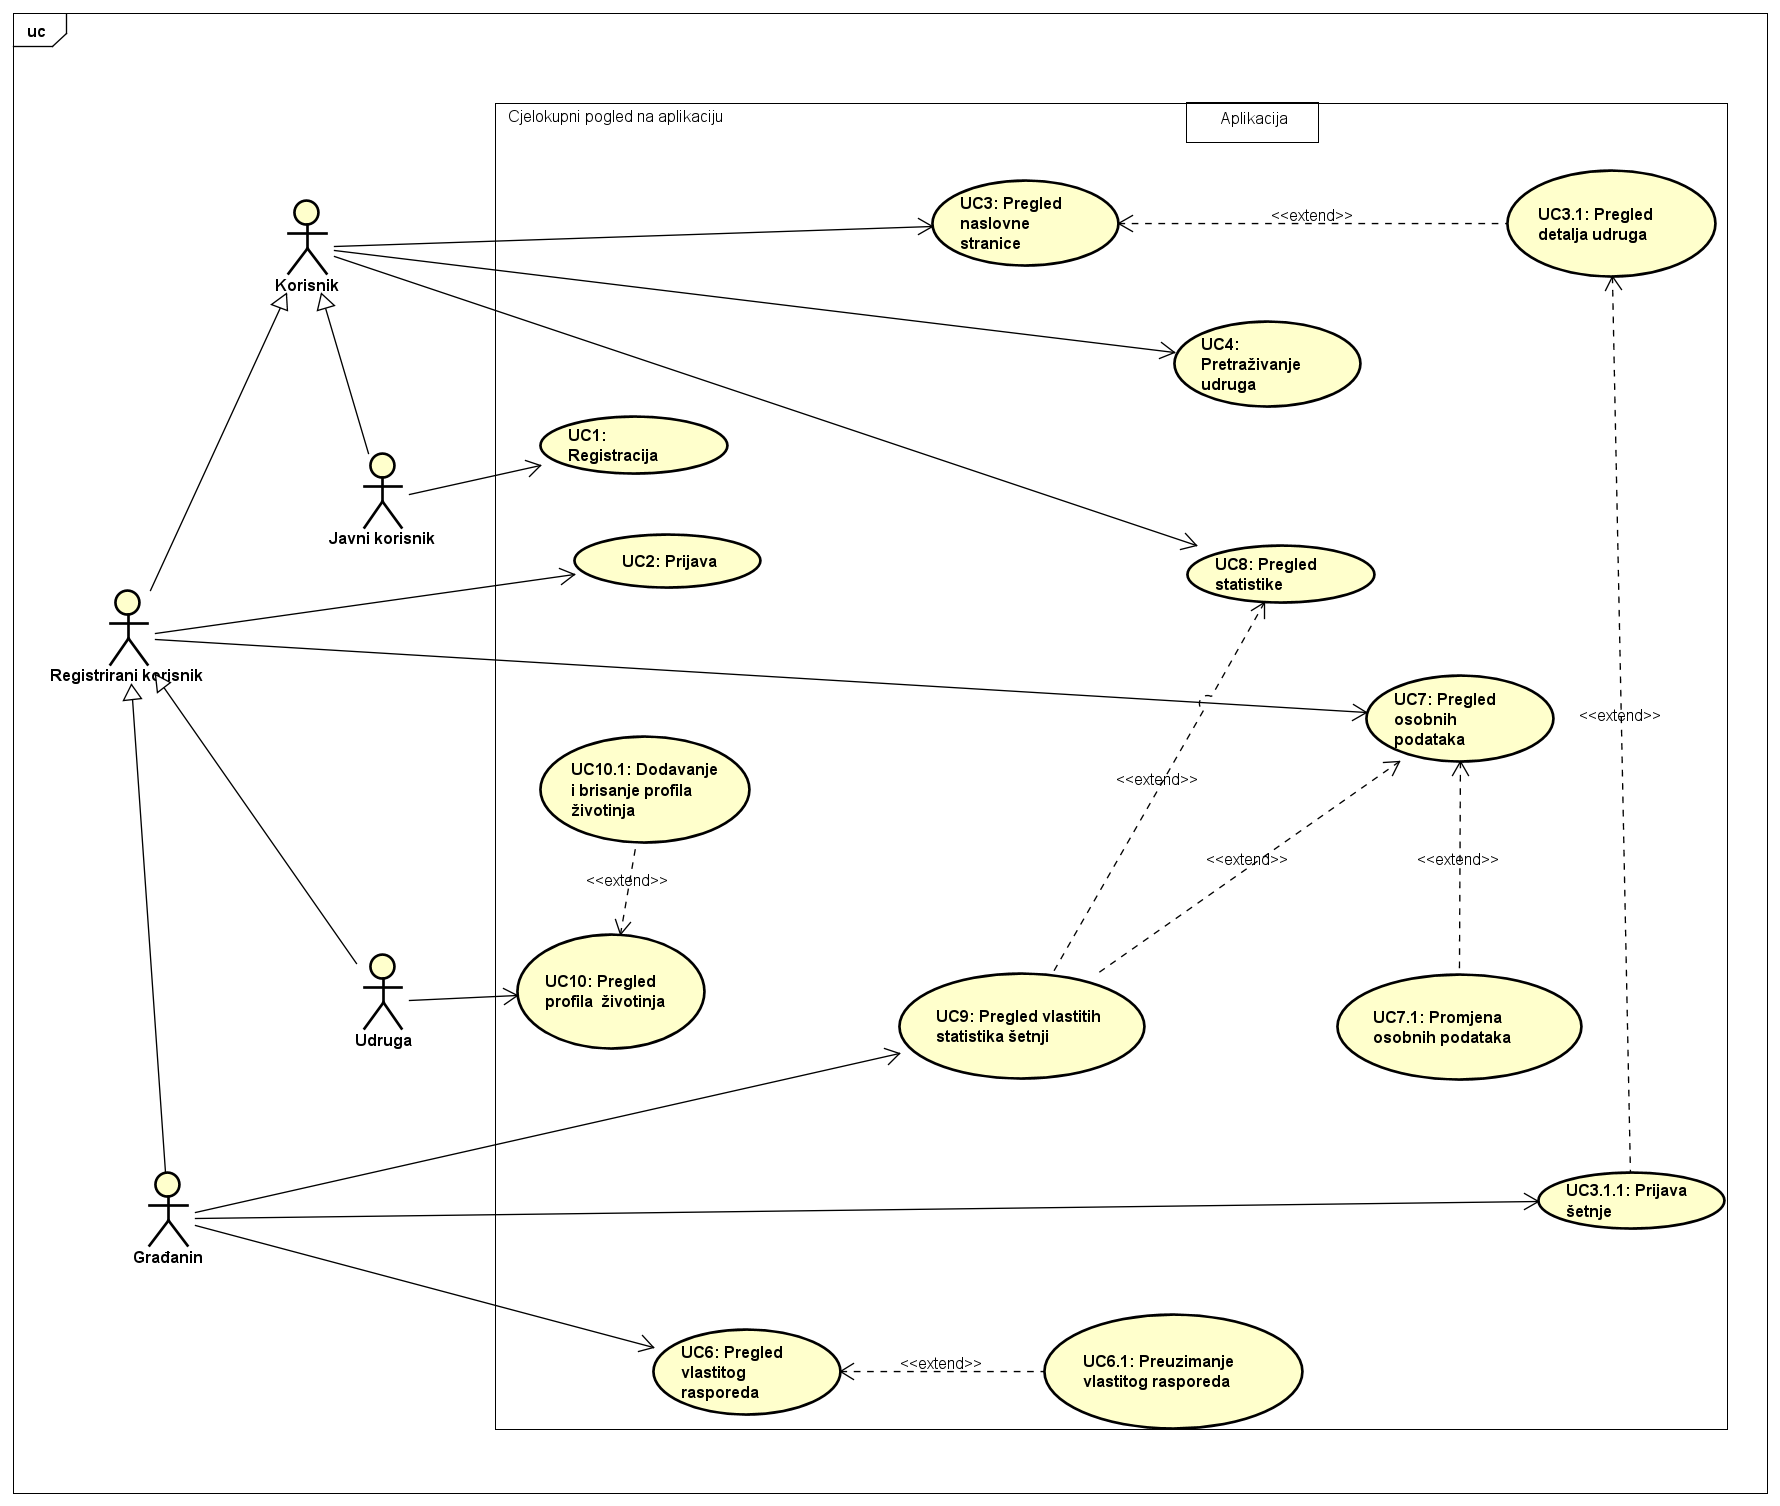
\includegraphics[width=\linewidth]{slike/UML.png}
						\centering
						\caption{Dijagram svih obrasca uporabe}
						\label{fig:uml}
					\end{figure}
					
				\eject		
				
			\subsection{Sekvencijski dijagrami}
				\noindent\textbf{Obrazac uporabe UC5 - Prijava šetnje}\\
				
				\noindent Građanin pregledom Udruge te odabirom željenog termina, šalje zahtjev za prikaz dostupnih životinja
				u terminu. Poslužitelj dohvaća sve slobodne životinje u odabranom terminu iz baze podataka, te ih 
				prikazuje. Ako je Građanin zadovoljan odabirom slobodnih životinja, odabire željeni oblik šetnje.
				Zatim se životinje filtriraju po odabranoj vrsti šetnje i prikazuju. Građanin odabire željene 
				životinje za termin. Kada je Građanin zadovoljan s odabirom, može poslati zahtjev za potvrdu 
				šetnje. Potvrdom šetnje se zauzima termin životinja te se prikazuje poruka "Šetnja prijavljena".
				
				\begin{figure}[H]
					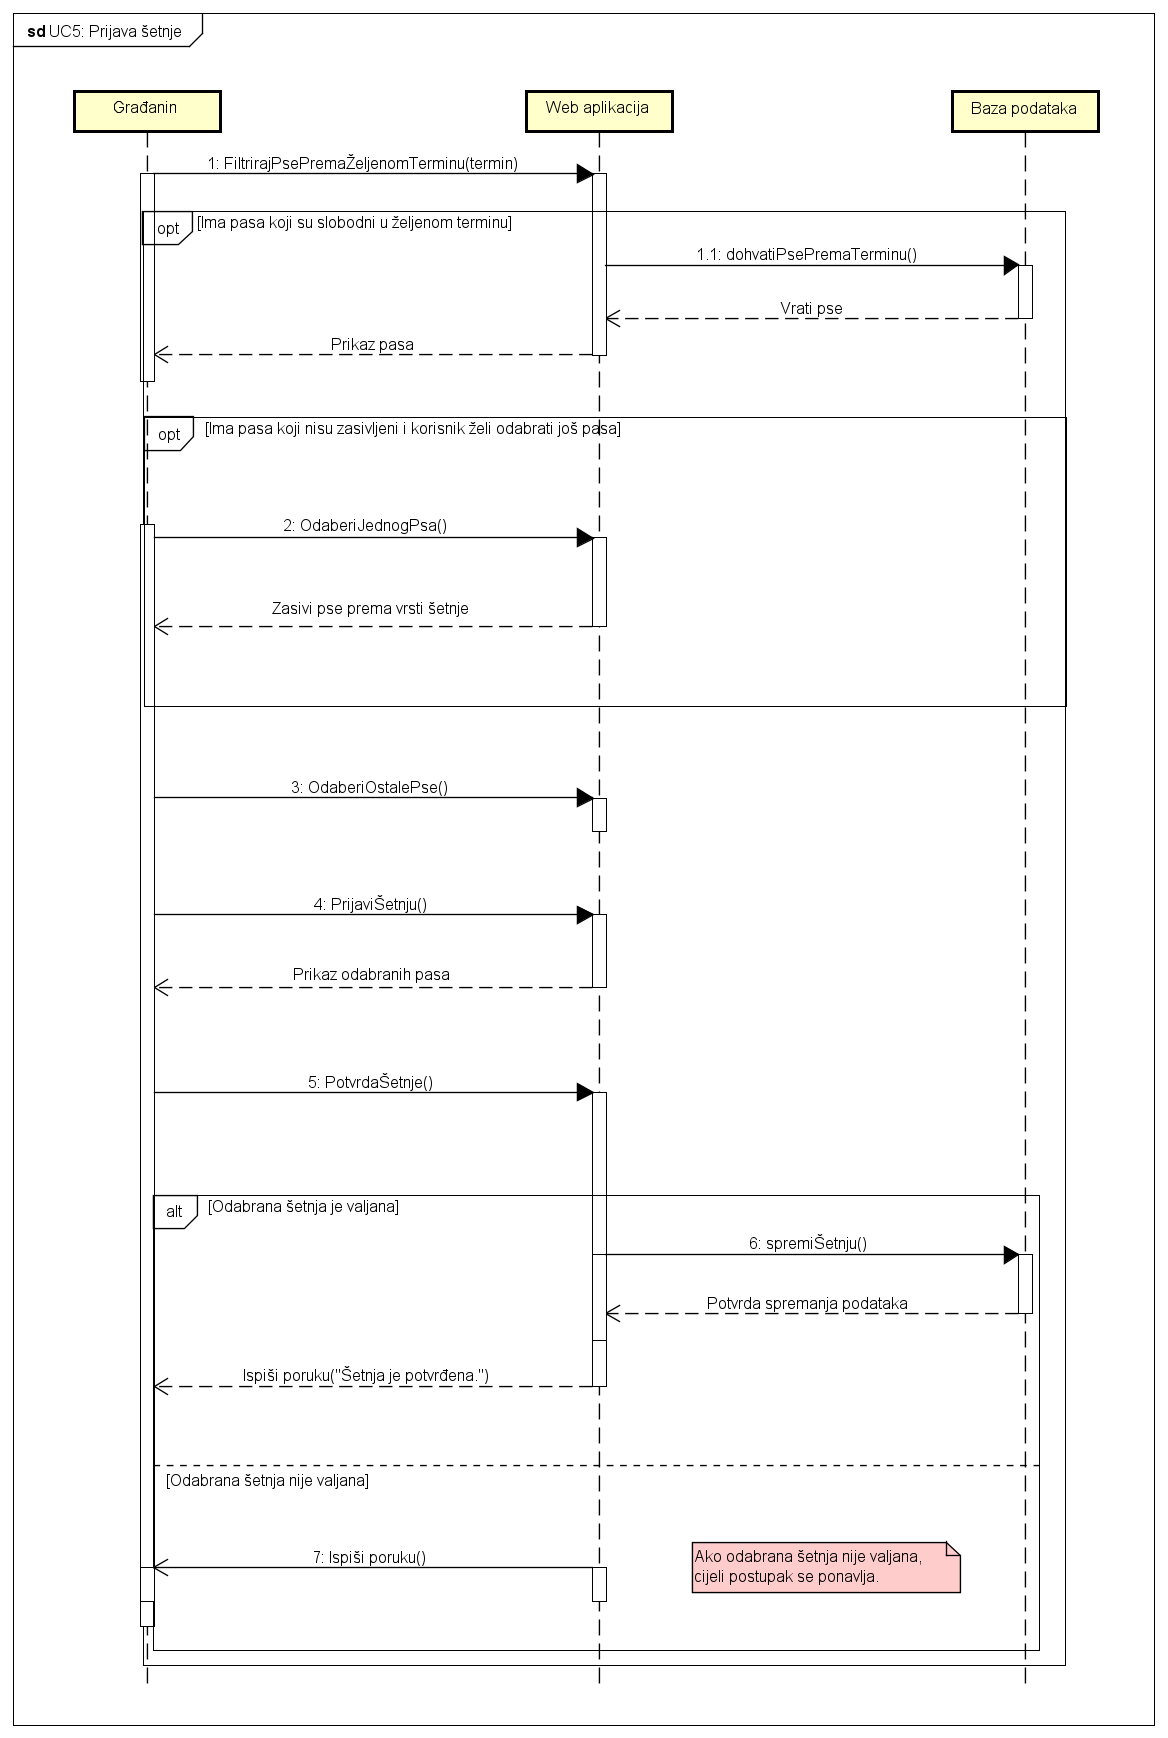
\includegraphics[width=\linewidth]{slike/SEK-5.png}
					\centering
					\caption{Sekvencijski dijagram za UC5}
					\label{fig:sek-5}
				\end{figure}
			
				\pagebreak
				\noindent\textbf{Obrazac uporabe UC6 i UC6.1 - Pregled i preuzimanje vlastitog rasporeda}\\
				
				\noindent Građanin šalje zahtjev za pregled vlastitog rasporeda. Poslužitelj dohvaća raspored 
				te mu ga prikazuje. Građanin je u mogućnosti odabirom opcije "Preuzmi vlasititi raspored" 
				zatražiti preuzimanje vlastitog raspored u PDF formatu.
				
				\begin{figure}[H]
					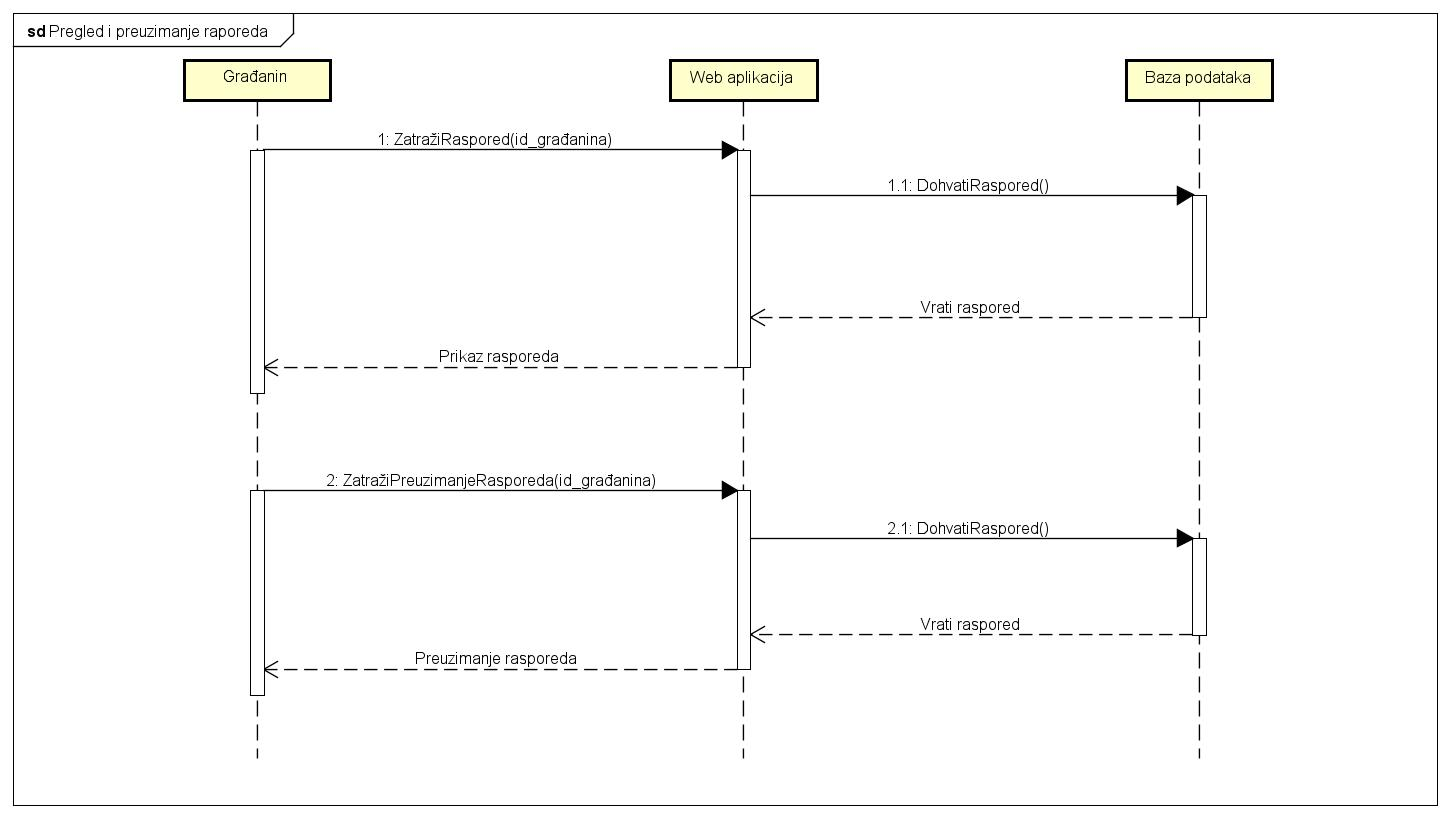
\includegraphics[width=\linewidth]{slike/SEK-6-6.1.jpg}
					\centering
					\caption{Sekvencijski dijagram za UC6 i UC6.1}
					\label{fig:sek-6-6.1}
				\end{figure}
				
				\eject
	
		\section{Ostali zahtjevi}
			 
			 
			 
			 \begin{packed_item}
			 	
			 	\item Sustav treba biti intuitivan i jednostavan za korištenje korisnicima koji prvi put koriste aplikaciju.
			 	\item Sustav mora omogućiti pristup i rad više korisnika istovremeno.
			 	\item Sustav treba biti implementiran kao web aplikacija i mora mu biti omogućen pristup iz javne mreže pomoću HTTPS protokola.
			 	\item Neregularne aktivnosti unutar sustava ne smiju narušiti njegov rad i daljnje normalno funkcioniranje.
			 	\item Sustav mora podržavati hrvatska slova (dijakritičke znakove).
			 	\item Baza podataka mora biti zaštićena, brza i otporna na moguće pogrešne zahtjeve.
			 	\item Dohvaćanje podataka iz baze ne smije trajati duže od nekoliko sekundi. 
			 	\item Sustav treba biti moguće nadograđivati, unaprijeđivati i razvijati bez narušavati postojećih funkcionalnosti.
			 	\item Prilikom prijave šetnje njezino trajanje mora biti zaokruženo na puni sat.
			 	\item Statistika prikazuje podatke stare do 30 dana.
			 	\item Datum mora biti u obliku dd-mm-yyyy.
			 	
			 \end{packed_item}


			 
			 
			 
	
	\chapter{Arhitektura i dizajn sustava}
		
		Projekt kao cjelina sastoji se od sljedećih podsustava:
		
		\begin{enumerate}
			\item  Web poslužitelja
			
			\item  Web aplikacije
			
			\item  Baze podataka
			
		\end{enumerate}
	
		\textbf{Web preglednik} je program koji omogućuje pregled web-stranica i njihovih multimedijalnih sadržaja. Web preglednik prevodi jezik kojim je Web stranica pisana u jezik razumljiv korisniku te šalje korisničke zahtjeve web poslužitelju.
		
		\textbf{Web poslužitelj} je računalo koje pohranjuje web stranice i sadržaje potrebne za njezin prikaz (primjerice HTML dokumente, CSS stilove, JavaScript datoteke i fotografije). Njegova uloga je povezivanje web preglednika s web aplikacijom kako bi ju učinio dostupnom korisniku.
		
		\textbf{Web aplikacija} je program koji radi na poslužitelju, a izvodi se u web pregledniku kojem pruža grafičko korisničko sučelje. Kada korisnik zatraži izvođenje nekog dijela aplikacije, web preglednik taj zahtjev šalje web poslužitelju. Aplikacija izvodi zadatak na poslužitelju i generira rezultat koji poslužitelj šalje web pregledniku, gdje je rezultat vidljiv korisniku kao odgovor na njegov upit. Web aplikacija je povezana s \textbf{bazom podataka} iz koje dohvaća podatke, a ulogu posrednika u komunikaciji između poslužiteljske i klijentske strane ima REST API.\\
		
		
			
		Programski jezik koji smo odabrali za izradu naše web aplikacije je Java, zajedno s JavaSpring radnim okvirom i React front-end knjižnicom za izgradnju korisničkog sučelja te programskim jezikom TypeScript. Razvojna okruženja u kojima ćemo raditi su Eclipse/IntelliJ te Visual Studio Code.
		
			
		Arhitektura našeg sustava temeljit će se na MVC (Model-View-Controller) obrascu. JavaSpring radni okvir omogućuje korištenje MVC softverske arhitekture te gotove komponente za razvoj web aplikacija. Arhitektura zasnovana na MVC obrascu pruža mogućnost odvajanja pojedinih dijelova aplikacije u zasebne komponente, što omogućuje njihov nezavisan razvoj te na taj način olakšava procese optimiranja i održavanja aplikacije.\\\\
		
		
		\textbf{MVC} obrazac softverske arhitekture sastoji se od:
			\begin{enumerate}
				\item  \textbf{Model} -Sadrži podatke, logike i funkcije ugrađene u program, upravlja njima te kao takva čini središnji dio sustava.
				
				\item  \textbf{View} -Predstavlja prikaz podataka (primjerice obrazac, tablica ili dijagram). Iste podatke je moguće prikazati na više različitih načina.
				
				\item  \textbf{Controller} -Upravlja korisničkim zahtjevima tako što pruža vanjsko sučelje web aplikacije u obliku RESTful web usluge (REST API-ja), prihvaća HTTP zahtjeve, poziva odgovarajuće usluge na sloju usluge te vraća odgovore klijentu u obliku JSON datoteke.\\
			\end{enumerate}
		
				
		\section{Baza podataka}
			
			\noindent Za pohranjivanje podataka koristimo relacijsku bazu podataka, konkretno PostgreSQL. 
			Baza podataka sadrži sljedeće entitete:
				
				\begin{packed_item}
					\item Korisnik
					\item Građanin
					\item Udruga
					\item Mjesto
					\item Životinja
					\item Vrsta
					\item Šetnja
					\item Šetnja Životinja
				\end{packed_item}
		
			\subsection{Opis tablica}
				
				\noindent\textbf{Korisnik}  Ovaj entitet sadržava sve informacije za prijavu Građanina i Udruga u sustav. Sadrži atribute: ID, KorisničkoIme, Email, Slika, Lozinka, BrojMobitela. Ovaj 
				entitet je u \textit{One-To-One} vezi s Građaninom i Udrugom preko atributa ID.
				\begin{longtabu} to \textwidth {|X[6, l]|X[6, l]|X[20, l]|}
					
					\hline \multicolumn{3}{|c|}{\textbf{Korisnik}}	 \\[3pt] \hline
					\endfirsthead
					
					\hline \multicolumn{3}{|c|}{\textbf{Korisnik}}	 \\[3pt] \hline
					\endhead
					
					\hline 
					\endlastfoot
					
					\cellcolor{LightGreen} ID & INT	&  	jedinstveni identifikator korisnika 	\\ \hline
					Korisničko ime	& VARCHAR &  korisničko ime korisnika \\ \hline 
					Email & VARCHAR &  e-mail adresa korisnika \\ \hline 
					Slika & LONGBLOB	&  slika profila korisnika		\\ \hline 
					Lozinka & VARCHAR	&  hash lozinke		\\ \hline 
					Broj mobitela & VARCHAR	&  broj mobitela korisnika		\\ \hline 
					
					
				\end{longtabu}
				
				\noindent\textbf{Građanin}  Ovaj entitet sadržava sve informacije vezane za Građanina. Sadrži atribute: ID, ID korisnika, Ime, Prezime. Ovaj entitet je u \textit{One-To-One} vezi s Korisnikom preko atributa ID korisnika, te u \textit{One-To-Many} vezi sa Šetnjom preko atributa ID.
				\begin{longtabu} to \textwidth {|X[6, l]|X[6, l]|X[20, l]|}
					
					\hline \multicolumn{3}{|c|}{\textbf{Građanin}}	 \\[3pt] \hline
					\endfirsthead
					
					\hline \multicolumn{3}{|c|}{\textbf{Građanin}}	 \\[3pt] \hline
					\endhead
					
					\hline 
					\endlastfoot
					
					\cellcolor{LightGreen} ID & INT	&  	jedinstveni identifikator građanina 	\\ \hline
					\cellcolor{LightBlue} ID korisnika	& INT &  jedinstveni identifikator korisnika (korisnik.ID) \\ \hline 
					Ime & VARCHAR &  ime građanina \\ \hline 
					Prezime & VARCHAR	&  prezime građanina		\\ \hline 
					
					
				\end{longtabu}
			
				\noindent\textbf{Udruga}  Ovaj entitet sadržava sve informacije vezane za Udrugu. Sadrži atribute: ID, ID korisnika, Oib, Ime, Adresa, ID mjesta. Ovaj entitet je u \textit{One-To-One} vezi s Korisnikom preko atributa ID korisnika. Entitet je također u \textit{One-To-Many} vezi sa Šetnjom preko atributa ID, te u \textit{Many-To-One} vezi s Mjestom preko atributa ID mjesta.
				\begin{longtabu} to \textwidth {|X[6, l]|X[6, l]|X[20, l]|}
					
					\hline \multicolumn{3}{|c|}{\textbf{Udruga}}	 \\[3pt] \hline
					\endfirsthead
					
					\hline \multicolumn{3}{|c|}{\textbf{Udruga}}	 \\[3pt] \hline
					\endhead
					
					\hline 
					\endlastfoot
					
					\cellcolor{LightGreen} ID & INT	&  	jedinstveni identifikator udruge \\ \hline
					\cellcolor{LightBlue} ID korisnika	& INT &  jedinstveni identifikator korisnika (korisnik.ID) \\ \hline 
					OIB & CHAR &  OIB udruge\\ \hline 
					Ime & VARCHAR &  ime udruge \\ \hline 
					Adresa & VARCHAR	&  adresa udruge		\\ \hline 
					\cellcolor{LightBlue} ID mjesta	& INT &  jedinstveni identifikator mjesta (mjesto.ID) \\ \hline 
					
					
				\end{longtabu}
			
				\noindent\textbf{Mjesto}  Ovaj entitet sadržava sve informacije vezane za Mjesto. Sadrži atribute: ID, Ime. Ovaj entitet je u \textit{One-To-Many} vezi s Udrugom preko atributa ID.
				\begin{longtabu} to \textwidth {|X[6, l]|X[6, l]|X[20, l]|}
					
					\hline \multicolumn{3}{|c|}{\textbf{Mjesto}}	 \\[3pt] \hline
					\endfirsthead
					
					\hline \multicolumn{3}{|c|}{\textbf{Mjesto}}	 \\[3pt] \hline
					\endhead
					
					\hline 
					\endlastfoot
					
					\cellcolor{LightGreen} ID & INT	&  	jedinstveni identifikator mjesta \\ \hline
					Ime & VARCHAR &  ime mjesta \\ \hline 
					
					
				\end{longtabu}
			
				\noindent\textbf{Životinja}  Ovaj entitet sadržava sve informacije vezane za Životinju. Sadrži atribute: ID, Slika, Opis, Ime, ID vrste, Godina rođenja, Preferirana vrsta šetnje, Spol, ID udruge. Ovaj entitet je u \textit{Many-To-One} vezi s Udrugom preko atributa ID udruge, te s Vrstom preko atributa ID vrste. Entitet je u \textit{Many-To-Many} vezi sa Šetnja Životinja preko atributa ID.
				\begin{longtabu} to \textwidth {|X[6, l]|X[6, l]|X[20, l]|}
					
					\hline \multicolumn{3}{|c|}{\textbf{Životinja}}	 \\[3pt] \hline
					\endfirsthead
					
					\hline \multicolumn{3}{|c|}{\textbf{Životinja}}	 \\[3pt] \hline
					\endhead
					
					\hline 
					\endlastfoot
					
					\cellcolor{LightGreen} ID & INT	&  	jedinstveni identifikator životinje \\ \hline
					Slika	& LONGBLOB &  slika životinje \\ \hline 
					Opis & VARCHAR &  opis životinje \\ \hline 
					Ime & VARCHAR &  ime životinje \\ \hline 
					\cellcolor{LightBlue} ID vrste	& INT &  jedinstveni identifikator vrste (vrsta.ID) \\ \hline 
					Godina rođenja & INT	&  godina rođenja životinje \\ \hline 
					Preferirana vrsta šetnje & VARCHAR & preferirana vrsta šetnje životinje \\ \hline
					Spol & VARCHAR & spol životinje \\ \hline
					\cellcolor{LightBlue} ID udruge & INT & jedinstveni identifikator udruge (udruga.ID) \\ \hline
					
				\end{longtabu}
			
				\noindent\textbf{Vrsta}  Ovaj entitet sadržava sve informacije vezane za Vrstu. Sadrži atribute: ID, Ime, Visina, Težina, Životni vijek, Grupa. Ovaj entitet je u \textit{One-To-Many} vezi sa Životinjom preko atributa ID.
				\begin{longtabu} to \textwidth {|X[6, l]|X[6, l]|X[20, l]|}
					
					\hline \multicolumn{3}{|c|}{\textbf{Vrsta}}	 \\[3pt] \hline
					\endfirsthead
					
					\hline \multicolumn{3}{|c|}{\textbf{Vrsta}}	 \\[3pt] \hline
					\endhead
					
					\hline 
					\endlastfoot
					
					\cellcolor{LightGreen} ID & INT	&  	jedinstveni identifikator vrste \\ \hline
					Ime	& VARCHAR &  ime vrste \\ \hline 
					Visina & VARCHAR &  prosječna visina vrste \\ \hline 
					Težina & VARCHAR &  prosječna težina vrste \\ \hline 
					Životni vijek	& VARCHAR &  prosječni životni vijek vrste \\ \hline 
					Grupa & VARCHAR	&  grupa vrste \\ \hline 
					
				\end{longtabu}
			
				\noindent\textbf{Šetnja}  Ovaj entitet sadržava sve informacije vezane za Šetnju. Sadrži atribute: ID, Trajanje, Početak, Vrsta, ID korisnika. Ovaj entitet je u \textit{Many-To-One} vezi s Građaninom preko atributa ID građanina, te u \textit{One-To-Many} vezi sa Šetnja Životinja preko atributa ID.
				\begin{longtabu} to \textwidth {|X[6, l]|X[6, l]|X[20, l]|}
					
					\hline \multicolumn{3}{|c|}{\textbf{Šetnja}}	 \\[3pt] \hline
					\endfirsthead
					
					\hline \multicolumn{3}{|c|}{\textbf{Šetnja}}	 \\[3pt] \hline
					\endhead
					
					\hline 
					\endlastfoot
					
					\cellcolor{LightGreen} ID & INT	&  	jedinstveni identifikator šetnje \\ \hline
					Trajanje	& INT &  vremensko trajanje šetnje \\ \hline 
					Početak & DATETIME &  vrijeme početka šetnje \\ \hline 
					Vrsta šetnje & VARCHAR &  vrsta šetnje \\ \hline 
					\cellcolor{LightBlue} ID građanina & INT	&  jedinstveni identifikator građanina (građanin.ID) \\ \hline 
					
				\end{longtabu}
			
				\noindent\textbf{Šetnja Životinja}  Ovaj entitet sadržava sve informacije o odnosu Šetnje i Životinje. Sadrži atribute: ID, ID šetnje, ID životinje. Ovaj entitet je u \textit{Many-To-One} vezi sa Šetnjom preko atributa ID šetnje, te u \textit{Many-To-Many} vezi sa Životinjom preko atributa ID životinje.
				\begin{longtabu} to \textwidth {|X[6, l]|X[6, l]|X[20, l]|}
					
					\hline \multicolumn{3}{|c|}{\textbf{Šetnja Životinja}}	 \\[3pt] \hline
					\endfirsthead
					
					\hline \multicolumn{3}{|c|}{\textbf{Šetnja Životinja}}	 \\[3pt] \hline
					\endhead
					
					\hline 
					\endlastfoot
					
					\cellcolor{LightGreen} ID & INT	&  	jedinstveni identifikator šetnje životinje \\ \hline
					\cellcolor{LightBlue} ID šetnje & INT	&  jedinstveni identifikator šetnje (šetnja.ID) \\ \hline 
					\cellcolor{LightBlue} ID životinje & INT	&  jedinstveni identifikator životinje (životinja.ID) \\ \hline
					
				\end{longtabu}
			
			
			\subsection{Dijagram baze podataka}
				\begin{figure}[H]
					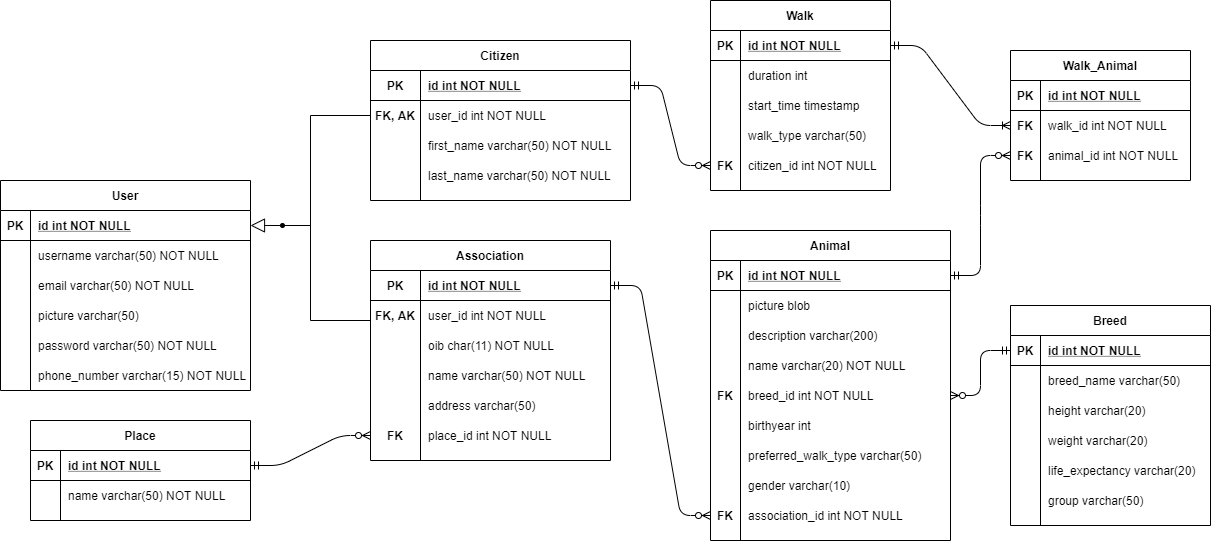
\includegraphics[width=\linewidth]{slike/ERD.png}
					\centering
					\caption{ER dijagram baze podataka}
					\label{fig:erd}
				\end{figure}
			
			\eject
			
			
		\section{Dijagram razreda}
		
			\begin{figure}[H]
				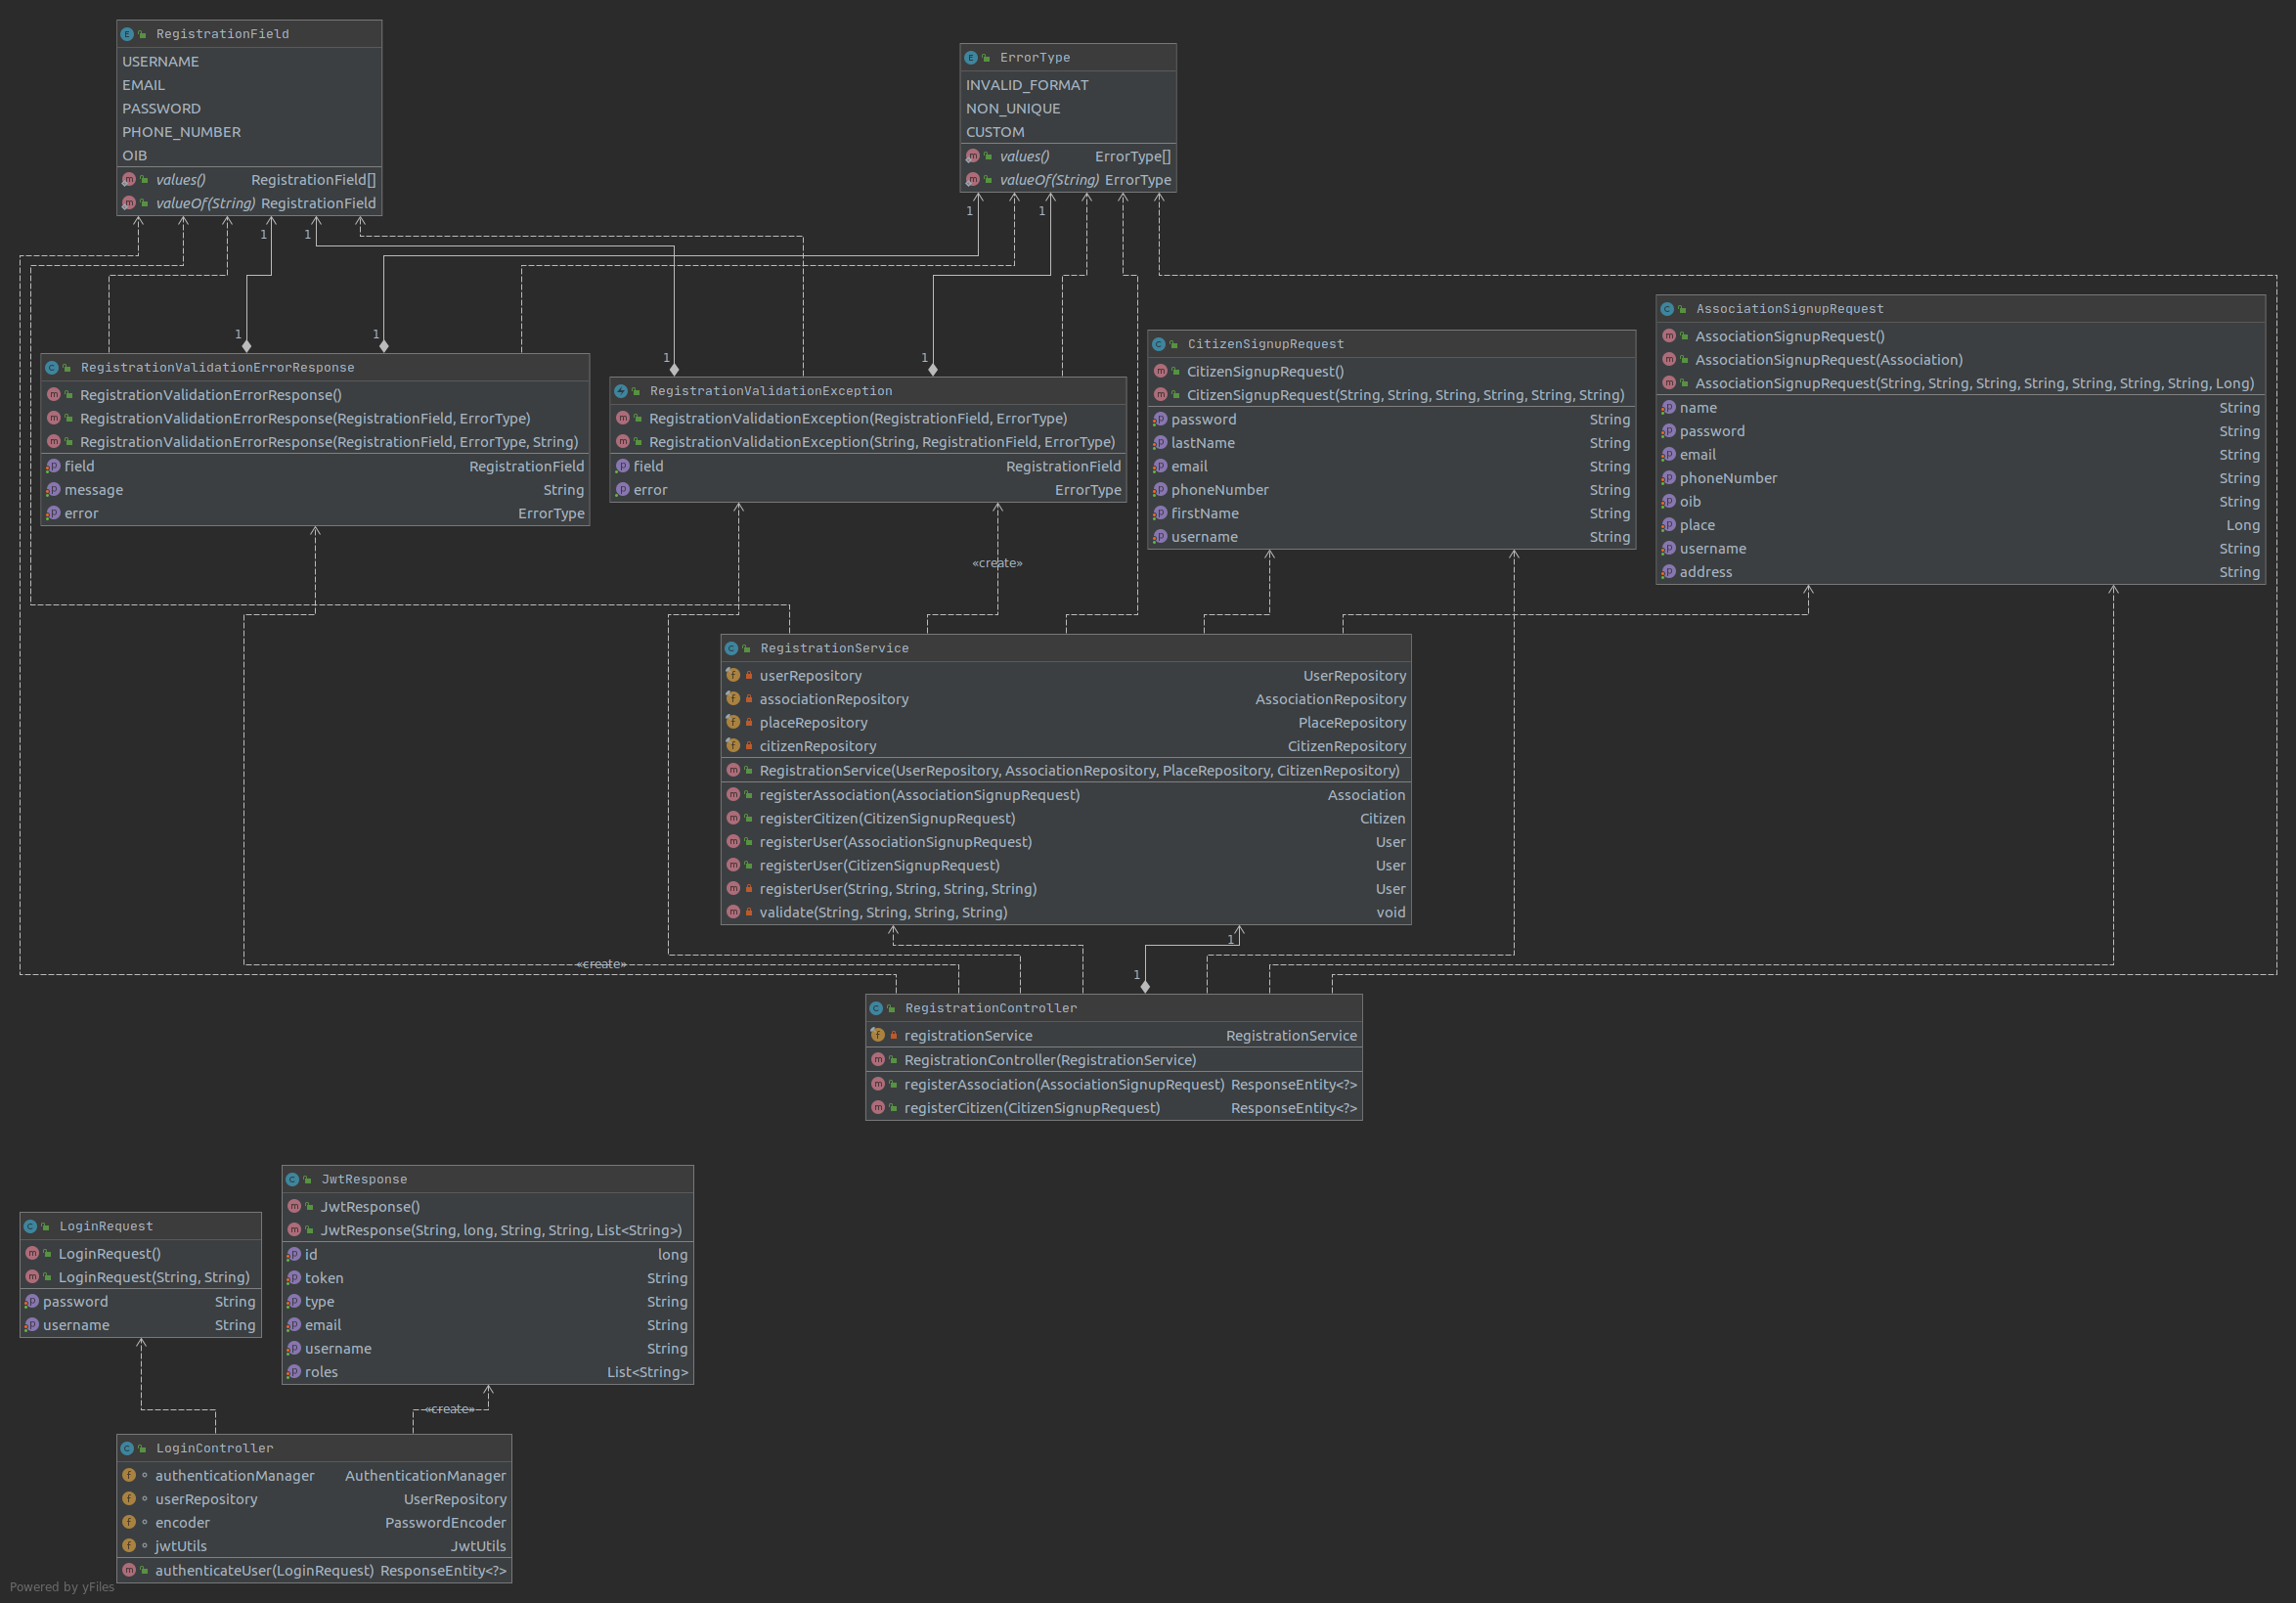
\includegraphics[width=\linewidth]{slike/Controllers-Services-Login-Registration.png}
				\centering
				\caption{Kontroleri i servisi za login i registraciju}
				\label{fig:controllers-services-login-registration}
			\end{figure}
		
			\begin{figure}[H]
				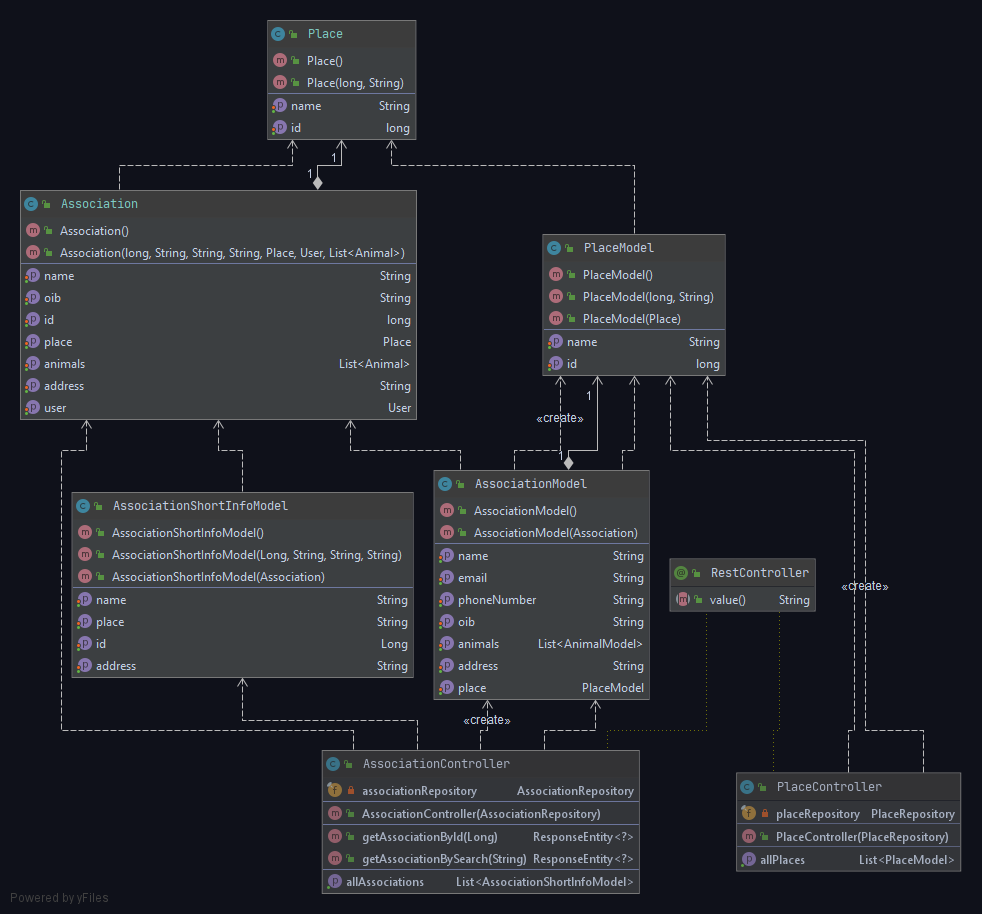
\includegraphics[width=\linewidth]{slike/Controllers-General.png}
				\centering
				\caption{Kontroleri za udruge i mjesta}
				\label{fig:controllers-general}
			\end{figure}
		
			\begin{figure}[H]
				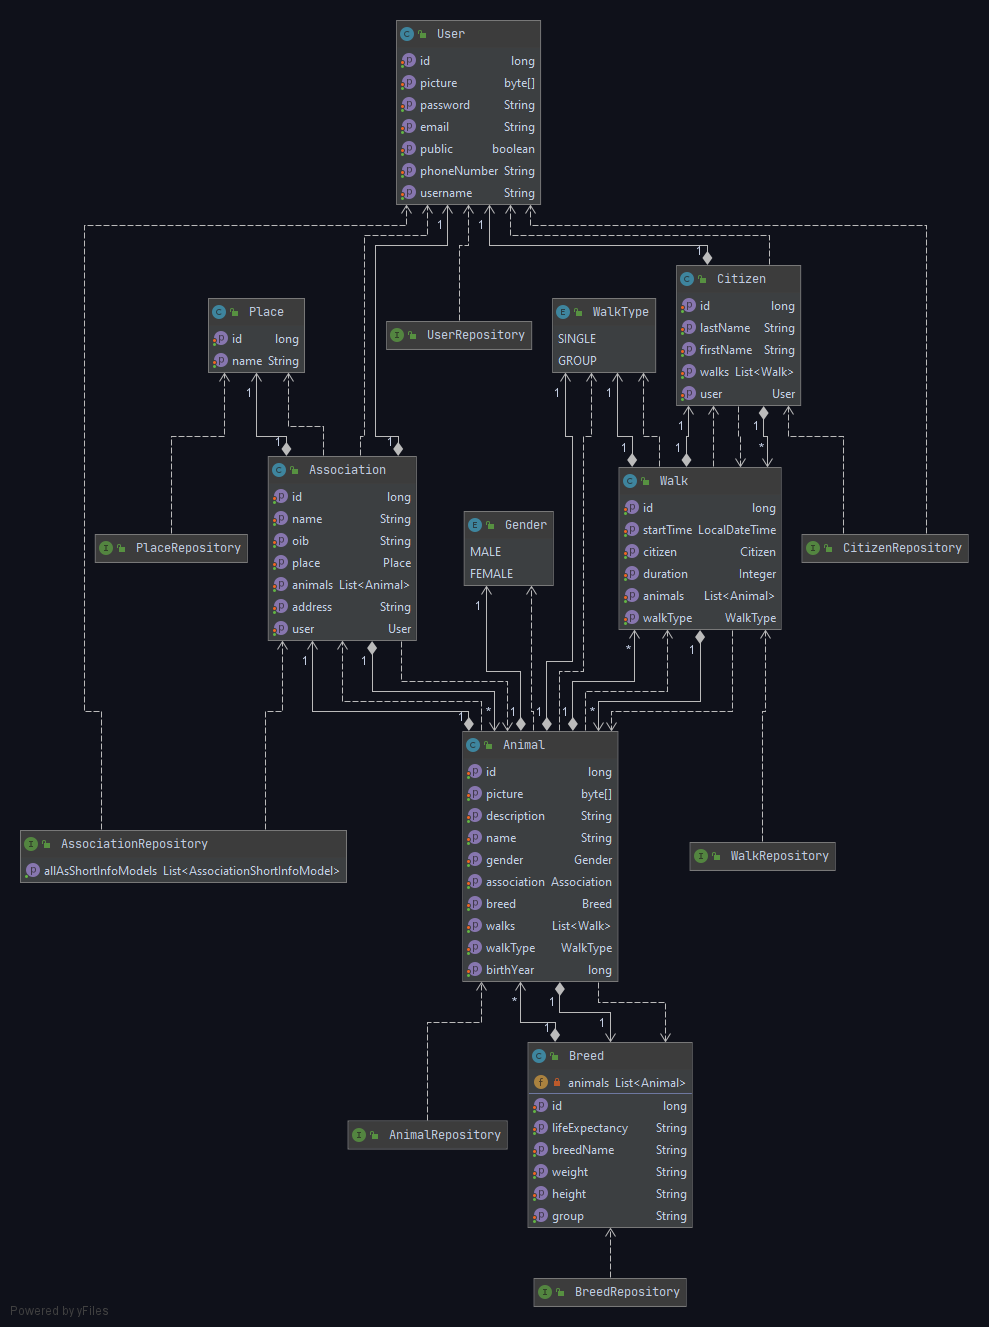
\includegraphics[width=\linewidth]{slike/Entities-Repositories.png}
				\centering
				\caption{Entiteti i repozitoriji}
				\label{fig:entities-repositories}
			\end{figure}
	
			\begin{figure}[H]
				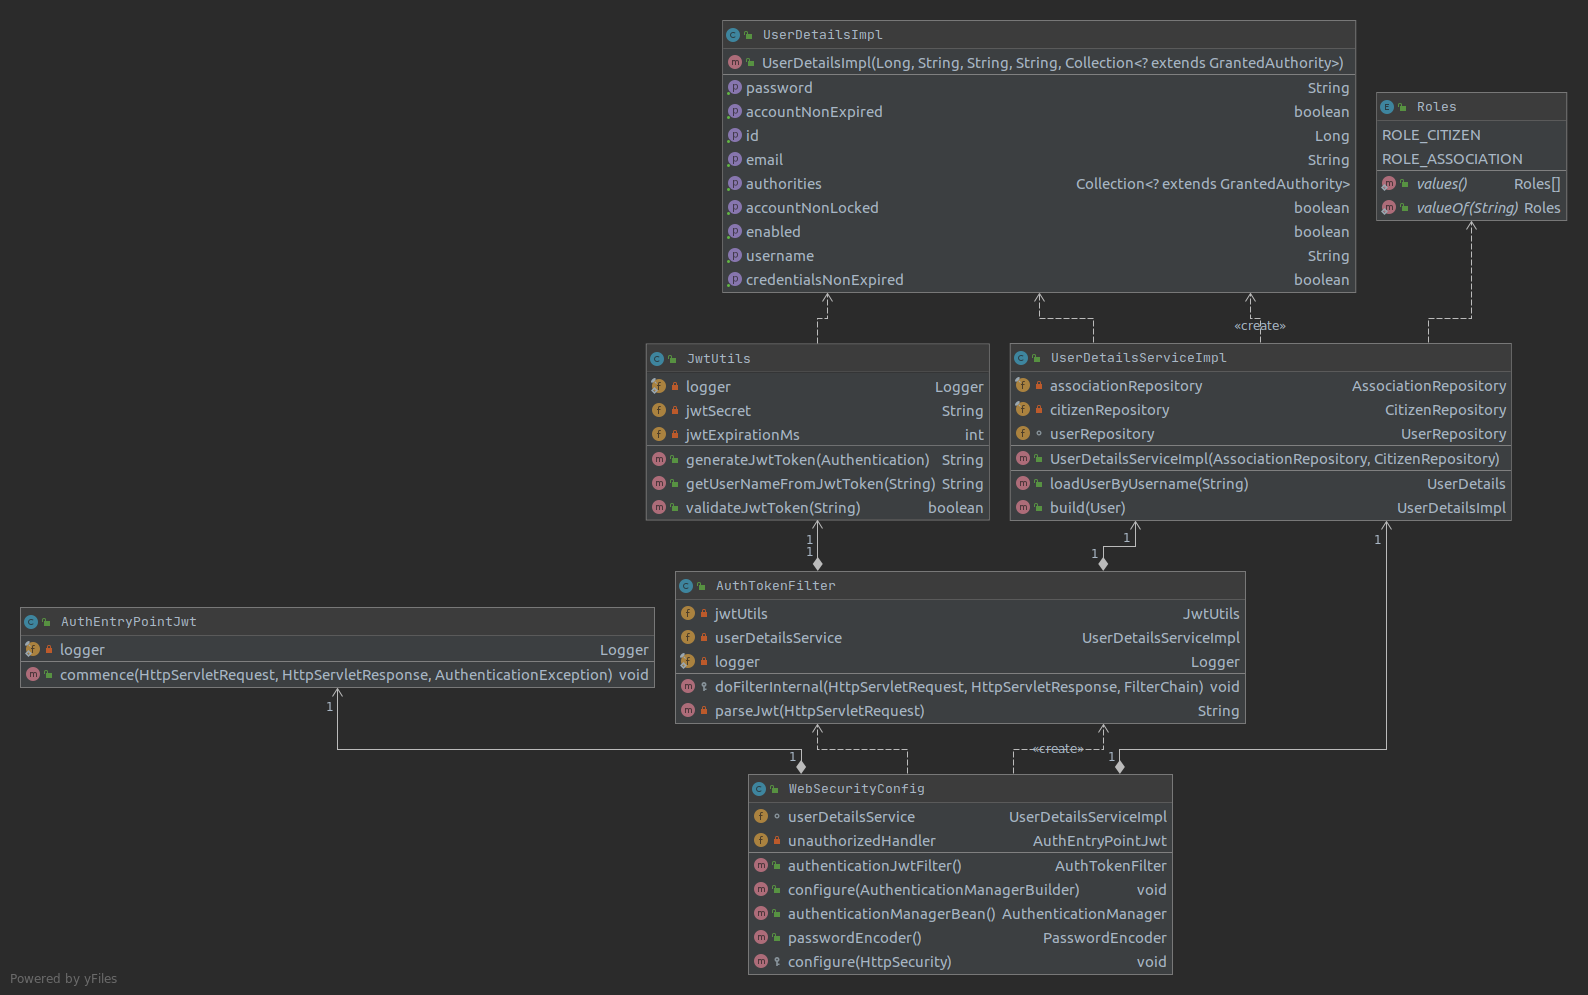
\includegraphics[width=\linewidth]{slike/Security.png}
				\centering
				\caption{Konfiguracija sigurnosti}
				\label{fig:security}
			\end{figure}
			
			\eject
			
			\begin{figure}[H]
				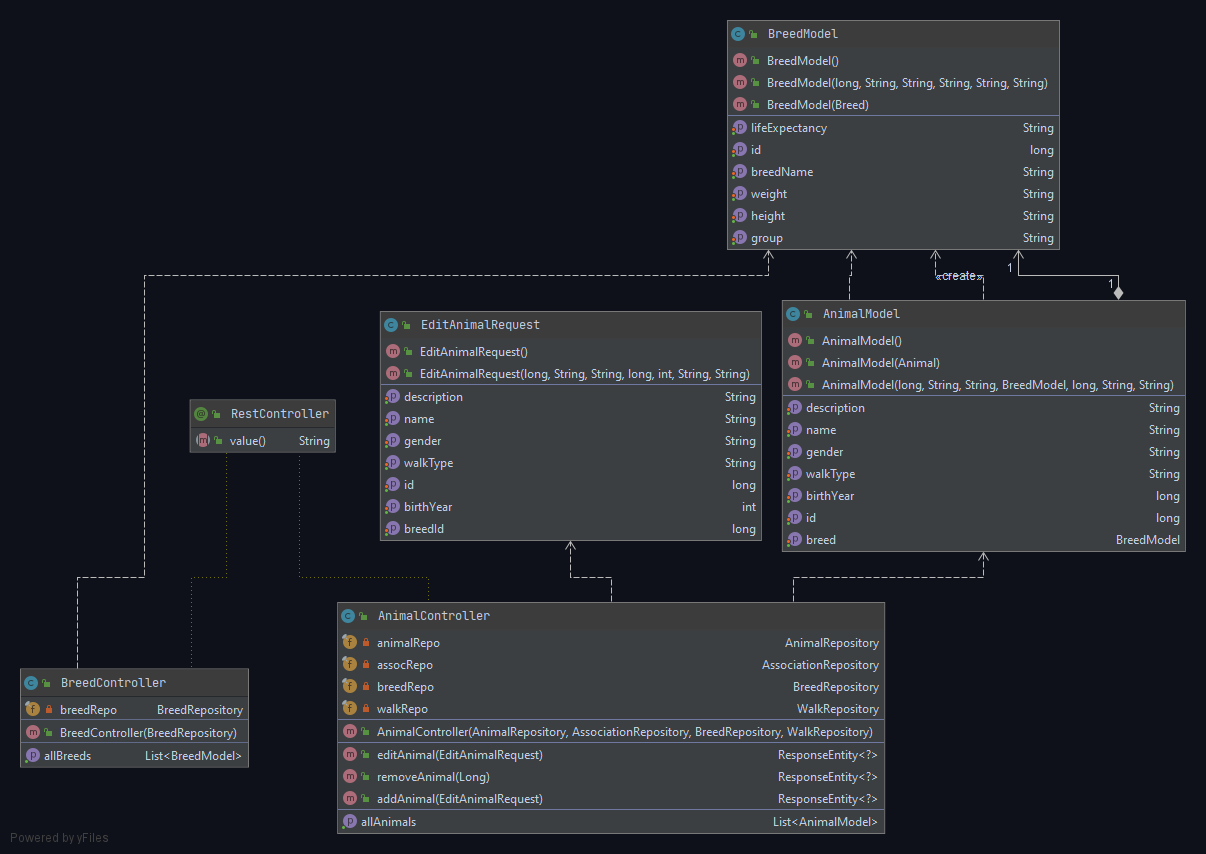
\includegraphics[width=\linewidth]{slike/AnimalController-BreedController.png}
				\centering
				\caption{Kontroleri za životinje i pasmine}
				\label{fig:animalcontroler-breedcontroller}
			\end{figure}
			
			\begin{figure}[H]
				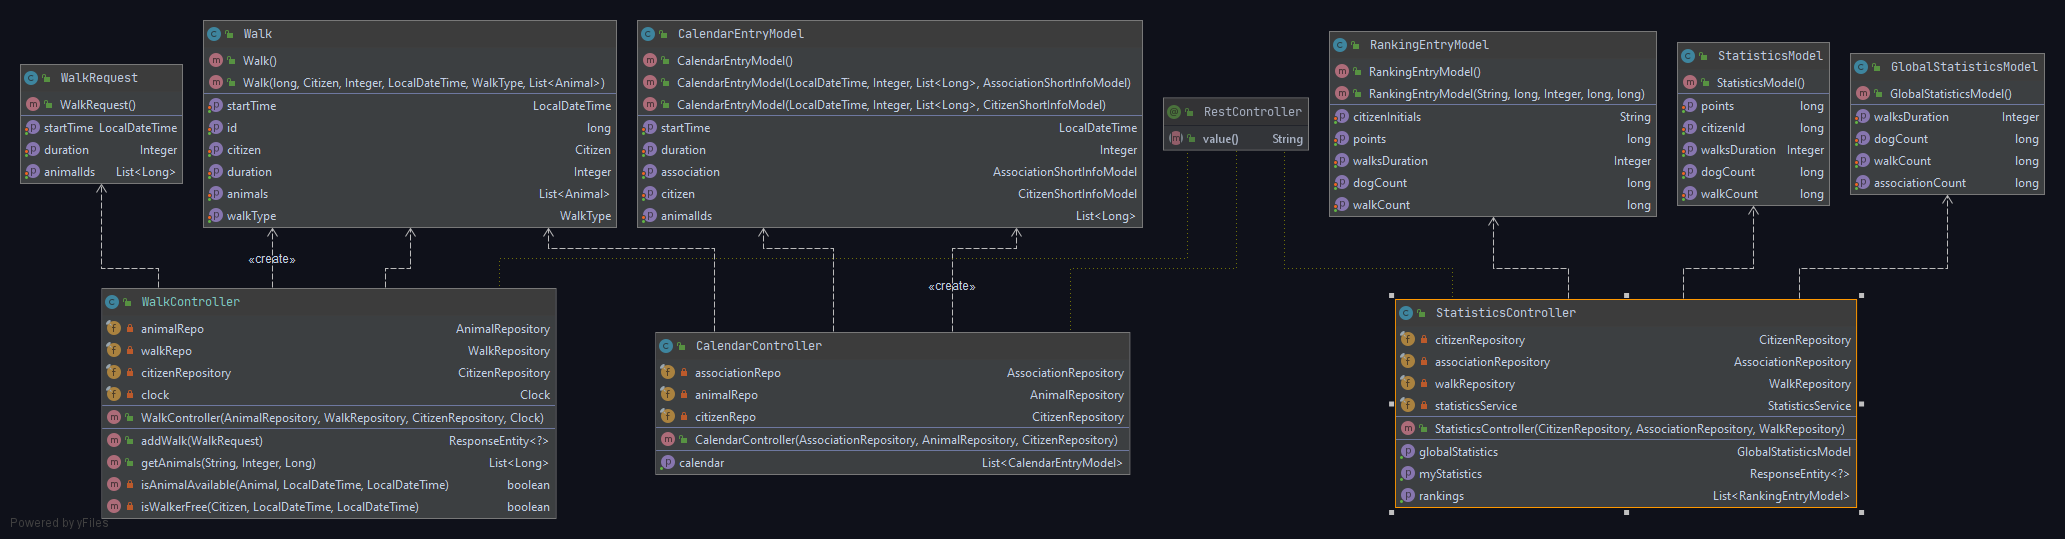
\includegraphics[width=\linewidth]{slike/WalkController-StatisticsController-CalendarController.png}
				\centering
				\caption{Kontroleri za šetnje, statistike i rasporede}
				\label{fig:walkcontroller-statisticscontroller-calendarcontroller}
			\end{figure}
			
			\eject
			
			\section{Dijagram stanja}
			\begin{figure}[H]
				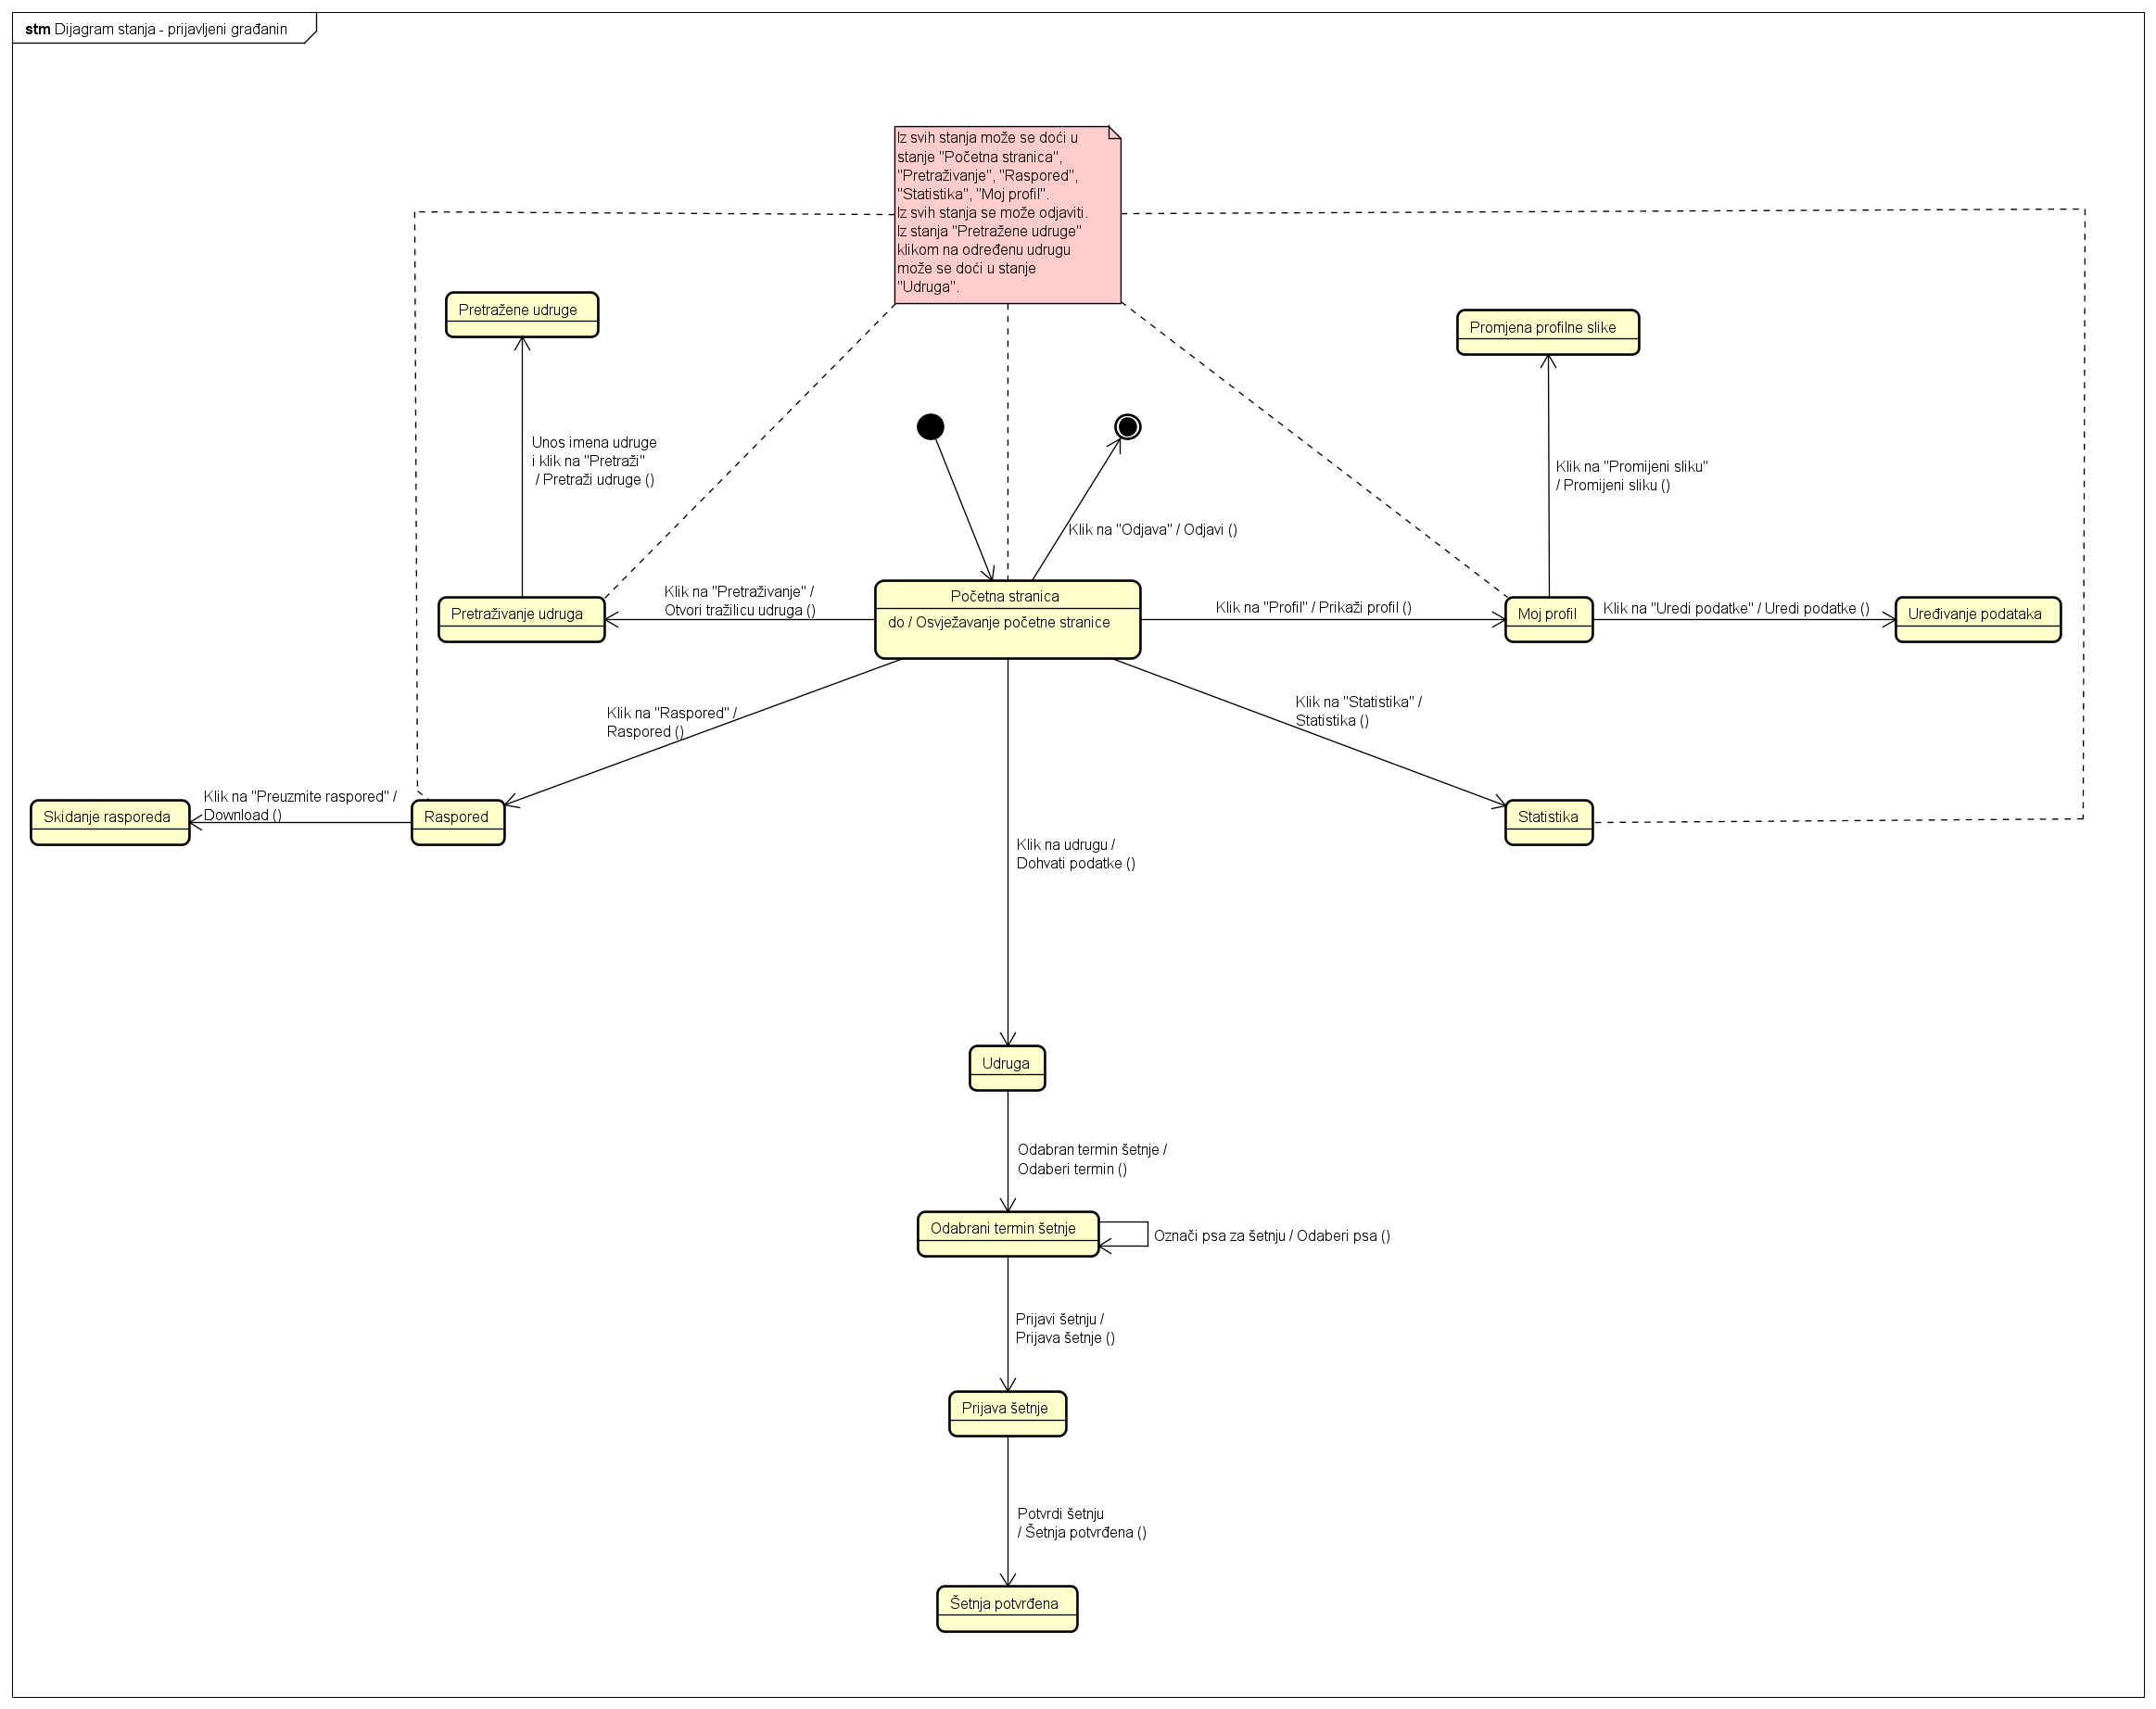
\includegraphics[width=\linewidth]{slike/D_stanja.png}
				\centering
				\caption{Dijagram stanja}
				\label{fig:dijagramstanja}
			\end{figure}
			
			\eject

			\section{Dijagram aktivnosti}
			\begin{figure}[H]
				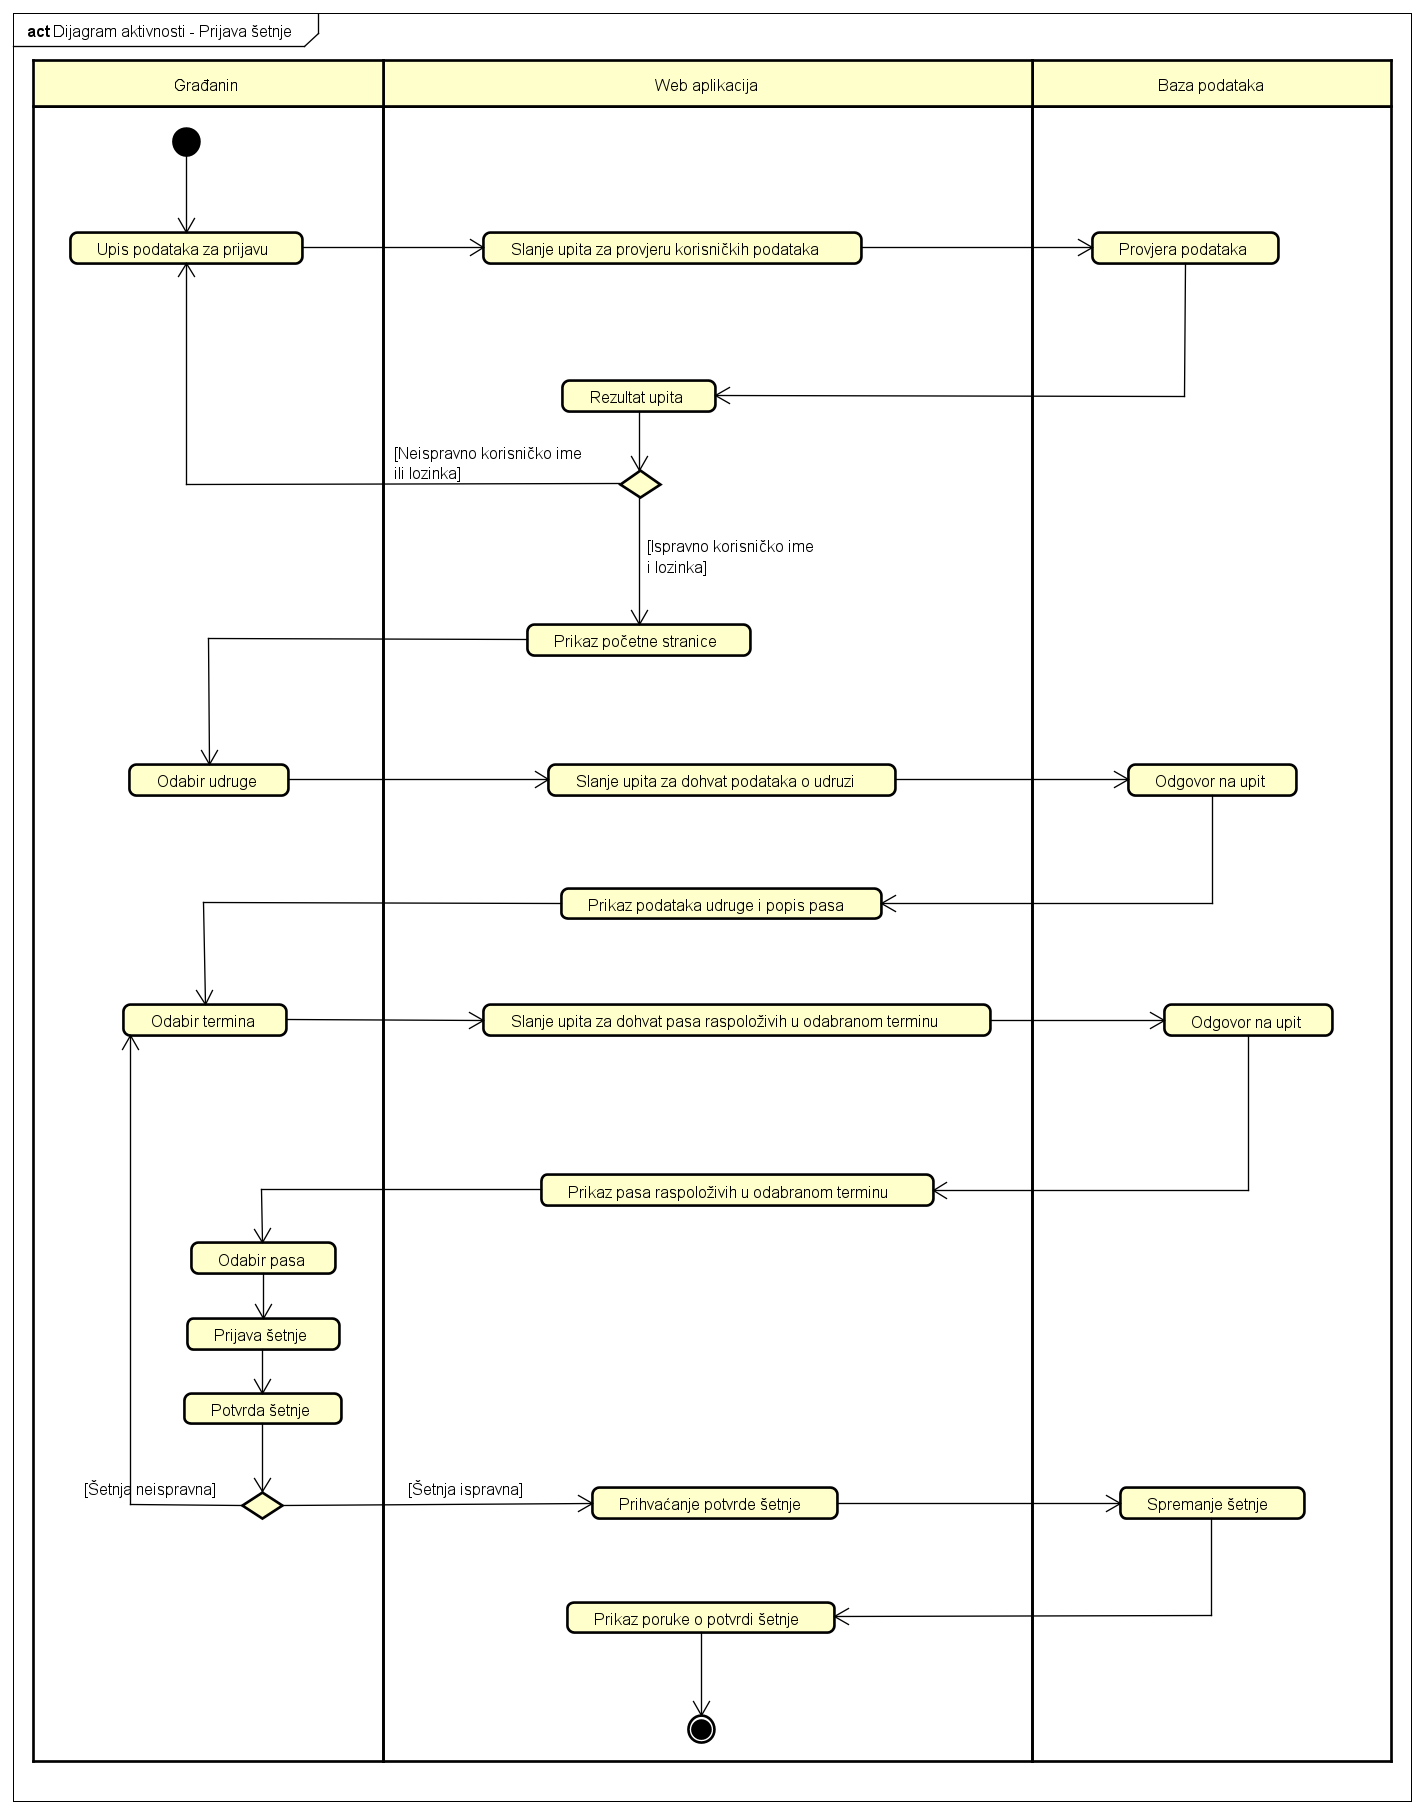
\includegraphics[width=\linewidth]{slike/D_akt.png}
				\centering
				\caption{Dijagram aktivnosti}
				\label{fig:dijagramaktivnosti}
			\end{figure}
			
			\eject
			
			\section{Dijagram komponenti}
			\begin{figure}[H]
				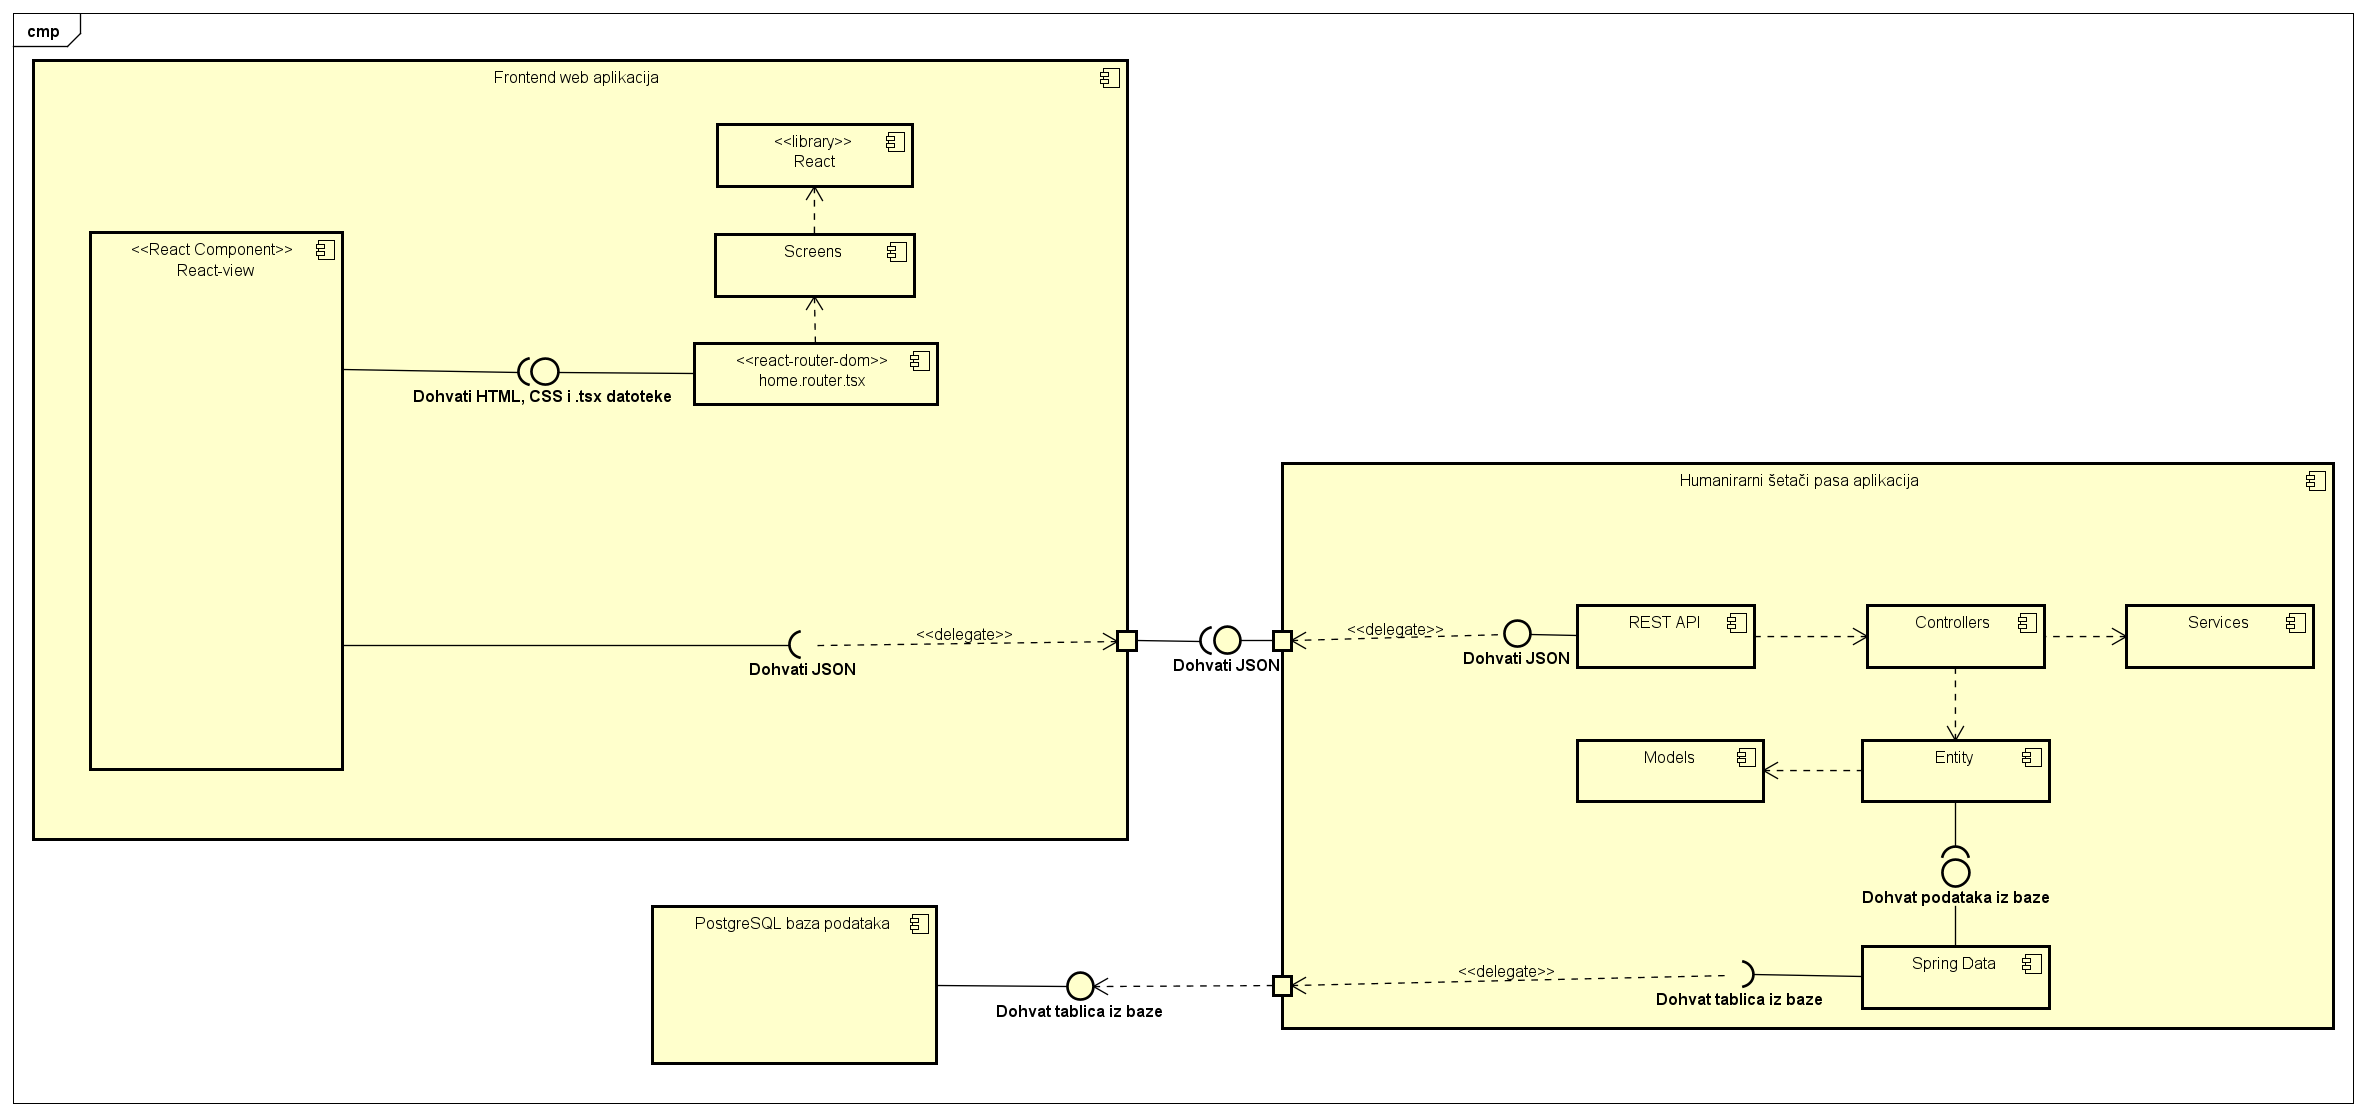
\includegraphics[width=\linewidth]{slike/ComponentDiagram3.png}
				\centering
				\caption{Dijagram komponenti}
				\label{fig:dijagramkomponenti}
			\end{figure}

	\chapter{Implementacija i korisničko sučelje}


\section{Korištene tehnologije i alati}

Za komunikaciju u timu korištene su aplikacije \underline{WhatsApp}\footnote{\url{https://www.whatsapp.com/}} i \underline{Discord}\footnote{\url{https://discord.com/}}. Na web platformi \underline{GitLab}\footnote{\url{https://gitlab.com}} nalazi se udaljeni repozitorij projekta, a kao sustav za upravljanje izvornim kodom korišten je \underline{Git}\footnote{\url{https://git-scm.com/}}. Za razvoj su korištena dva razvojna okruženja, \underline{Microsoft Visual Studio Code}\footnote{\url{https://visualstudio.microsoft.com/}} i \underline{Intellij IDEA}\footnote{\url{https://www.jetbrains.com/idea/}}. Microsoft Visual Studio Code je integrirano razvojno okruženje tvrtke Microsoft, a koristi se za razvoj računalnih programa, web stranica, web aplikacija, web usluga i mobilnih aplikacija. IntelliJ IDEA integrirano je razvojno okruženje napisano u Javi za razvoj računalnog softvera, razvio ga je JetBrains, a dostupan je kao izdanje licenci za zajednicu Apache 2 i u vlastitom komercijalnom izdanju. \par		
Aplikacija je napisana koristeći aplikacijski okvir \underline{Spring Framework}\footnote{\url{https://spring.io/}} i jezik \underline{Java}\footnote{\url{https://www.java.com/en/}} za izradu backenda. Spring je skup biblioteka i alata koji olakšava razvoj aplikacija te čini programiranje u Javi bržim, lakšim i sigurnijim. Usredotočenost Springa na brzinu, jednostavnost i produktivnost učinila ga je najpopularnijim okvirom za Javu. Za lakše uključivanje i integriranje modula, postavljanje securityja i mapiranje objektnog modela na relacijsku bazu podataka korišten je Spring Boot. \underline{Spring Boot  }\footnote{\url{https://spring.io/projects/spring-boot/}} radi automatsko podešavanja i povezivanje različitih modula tako da analizira što smo uključili u classpath te sam zaključuje kako te module povezati u smislenu cjelinu. Za razvoj Web servisa korišten je \underline{REST}. REST, ili REpresentational State Transfer, arhitekturalni je stil za razvoj Web servisa koji pruža standard između računalnih sustava na webu, olakšavajući njihovu međusobnu komunikaciju. \par
Za praćenje promjena u bazi podataka korišten je \underline{Liquibase}\footnote{\url{https://www.liquibase.org/}}. Liquibase je knjižnica sa neovisnom bazom podataka otvorenog koda za praćenje, upravljanje i primjenu promjena sheme baze podataka. Pokrenut je 2006. godine kako bi omogućio lakše praćenje promjena u bazama podataka. Sve promjene u bazi podataka pohranjuju se u tekstualne datoteke (XML, JSON) i identificiraju se kombinacijom oznake "id" i "author", kao i imenom same datoteke. Za upravljanje bazom podataka korišten je besplatan sustav \underline{PostgreSQL}\footnote{\url{https://www.postgresql.org/}} koji poštuje ACID principe pri izvođenju transakcija. Za testiranje backenda korišten je jednostavan okvir za pisanje ponovljivih testova \underline{JUnit}\footnote{\url{https://junit.org/}}. JUnit je instanca xUnit arhitekture za okvire za jedinstveno testiranje. \par
Za izradu frontenda korišten je JavaScript library \underline{React}\footnote{\url{https://reactjs.org/}} i jezik \underline{TypeScript}\footnote{\url{https://www.typescriptlang.org/}}. React se koristi za izgradnju korisničkog sučelja ili UI komponenti. Održava ga Facebook. React se može koristit kao osnova u razvoju aplikacija. Za realizaciju pojedinih prikaza kao što su okviri za prijavu i registraciju, tablice za statistiku, gumbi i slično, korišten je \underline{Material-UI}\footnote{\url{https://material-ui.com/}}. To je open-source projekt koji sadrži React komponente koje implementiraju Googleov Material Design. Za preuzimanje rasporeda šetnji korišten je React-pdf koji služi za jednostavno generiranje PDF datoteka. HTTP zahtjevi i odgovori ostvareni su korištenjem \underline{Axios-a}\footnote{\url{https://www.npmjs.com/package/axios}}. Axios je vrlo popularan JavaScript library za izvršavanje HTTP zahtjeva. Podržava starije i sve moderne preglednike, radi u Node.js-u te provodi automatsku transformaciju JSON podataka. Temelji se na obećanjima, što omogućuje pisanje async/await koda za vrlo lako izvršavanje XHR zahtjeva. Dizajn web aplikacije napravljen je pomoću stilskog jezika \underline{CSS}\footnote{\url{https://www.w3.org/Style/CSS/Overview.en.html}}. Testiranje frontenda ostvareno je koristeći radni okvir \underline{Selenium}\footnote{\url{https://www.selenium.dev/}}. \par
Dokumentacija je napisana u jeziku \underline{LaTex}\footnote{\url{https://www.latex-project.org/}} u integriranom okruženju za pisanje \underline{TeXStudio}\footnote{\url{https://www.texstudio.org/}}. Za izradu UML dijagrama korišten je alat \underline{Astah UML}\footnote{\url{https://astah.net/downloads/}}. ER dijagram baze podataka izrađen je u besplatnom online softveru \underline{draw.io}\footnote{\url{https://app.diagrams.net/}}, koji se između ostalog koristi i za izradu dijagrama toka i procesa, organizacijskih dijagrama, UML, ER i mrežnih dijagrama.



\eject 

\section{Ispitivanje programskog rješenja}

	\subsection{Ispitivanje komponenti}

	
	\noindent Za testiranje smo odabrali WalkController i AssociationController koji implementiraju glavne funkcionalnosti sustava. Testirali smo controllere kako bi provjerili rad sustava u cjelini. Prije testova postavljeni su testni podaci. Na slici je prikazano postavljanje Spring Boot Security podataka.

	\begin{figure}[H]
		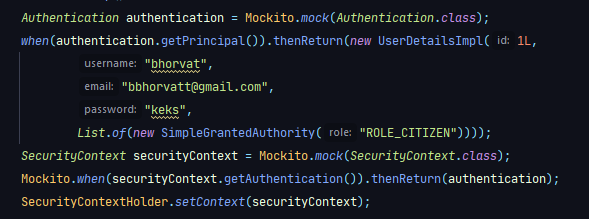
\includegraphics[width=\linewidth]{slike/Testovi-1.png}
		\centering
		\caption{Postavljanje sigurnosti}
		\label{fig:testovi1}
	\end{figure}

	\noindent Zbog testiranja prijave šetnje u prošlom vremenu, postavili smo fiksni datum kako je prikazano na slici dolje. Zbog vremenskih zona zahtjevi koji se šalju su u vremenskoj zoni GMT+0, a u sustavu se pohranjuju u vremenskoj zoni GMT+1.

	\begin{figure}[H]
		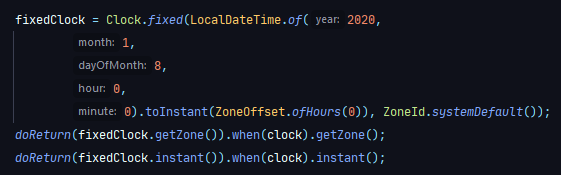
\includegraphics[width=\linewidth]{slike/Testovi-2.png}
		\centering
		\caption{Postavljanje fiksnog vremena}
		\label{fig:testovi2}
	\end{figure}

	\eject

	\noindent Zbog testiranja prijave šetnje kad je pas već zauzet, potrebna su nam dva građana.

	\begin{figure}[H]
		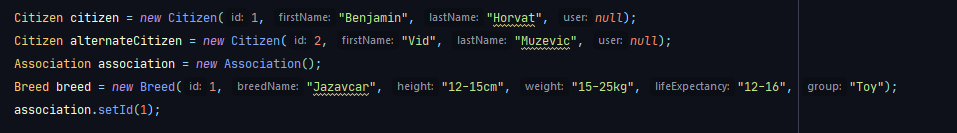
\includegraphics[width=\linewidth]{slike/Testovi-3.png}
		\centering
		\caption{Postavljanje 2 građana, 1 udruge i 1 pasmine}
		\label{fig:testovi3}
	\end{figure}

	\noindent Postavili smo testne podatke za dva psa koji su predodređeni za pojedinačnu šetnju i dva psa koji su predodređeni za grupnu šetnju. Zatim su postavljeni podaci za pet šetnji sa prije definiranim životinjama.

	\begin{figure}[H]
		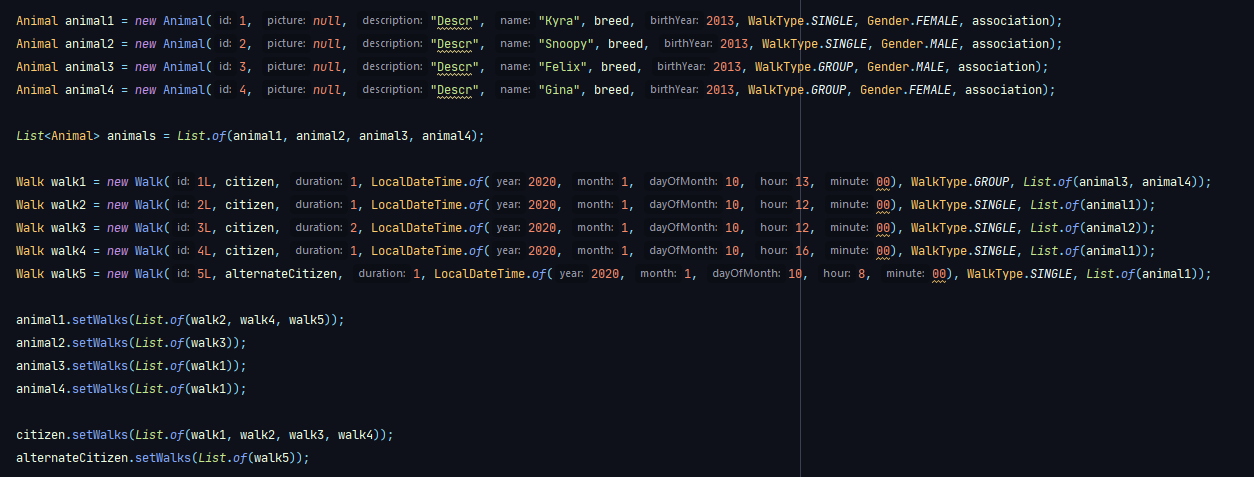
\includegraphics[width=\linewidth]{slike/Testovi-4.png}
		\centering
		\caption{Postavljanje životinja i šetnji}
		\label{fig:testovi4}
	\end{figure}
	
	\eject

	\noindent Postavljanje ponašanja dvojnika za navedene pozive metoda AnimalRepositoryja.

	\begin{figure}[H]
		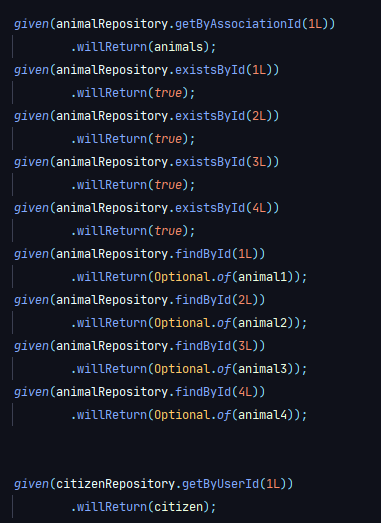
\includegraphics[width=\linewidth]{slike/Testovi-5.png}
		\centering
		\caption{Postavljanje dvojnika}
		\label{fig:testovi5}
	\end{figure}

	\noindent Na API poziv "/api/walk" šaljemo ispravne podatke šetnje. Očekivani rezultat je statusni kod 200.

	\begin{figure}[H]
		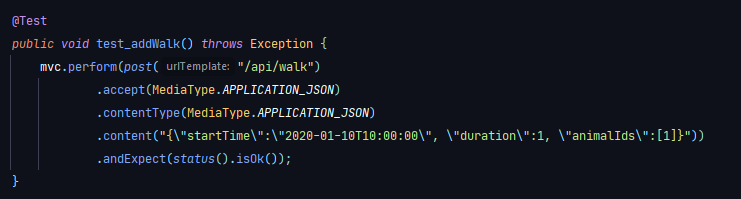
\includegraphics[width=\linewidth]{slike/Testovi-6.png}
		\centering
		\caption{Testiranje ispravne šetnje}
		\label{fig:testovi6}
	\end{figure}

	\noindent Na API poziv "/api/walk" šaljemo početak šetnje koji je prošao. Očekivani rezultat je statusni kod 400.

	\begin{figure}[H]
		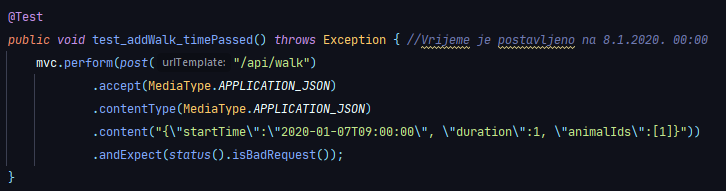
\includegraphics[width=\linewidth]{slike/Testovi-7.png}
		\centering
		\caption{Testiranje šetnje u prošlom vremenu}
		\label{fig:testovi7}
	\end{figure}
	
	\noindent Na API poziv "/api/walk" šaljemo podatke o šetnji u terminu u kojem je građanin već zauzet. Očekivani rezultat je statusni kod 400.

	\begin{figure}[H]
		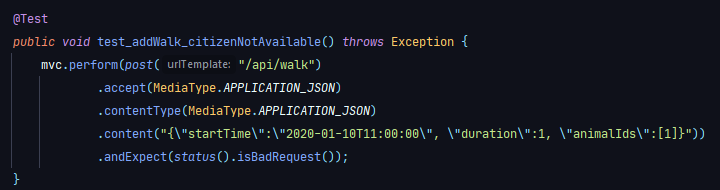
\includegraphics[width=\linewidth]{slike/Testovi-8.png}
		\centering
		\caption{Testiranje šetnje za koju građanin nije dostupan}
		\label{fig:testovi8}
	\end{figure}

	\noindent Na API poziv "/api/walk" šaljemo podatke o šetnji bez navedene životinje. Očekivani rezultat je statusni kod 400.

	\begin{figure}[H]
		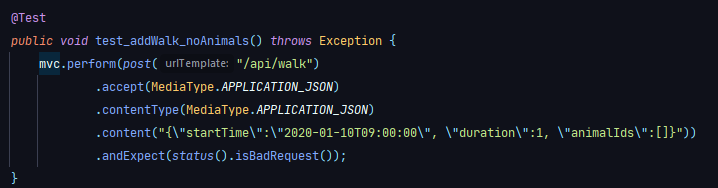
\includegraphics[width=\linewidth]{slike/Testovi-9.png}
		\centering
		\caption{Testiranje šetnje bez odabrane životinje}
		\label{fig:testovi9}
	\end{figure}

	\noindent Na API poziv "/api/walk" šaljemo podatke o šetnji u terminu u kojem je životinja već zauzeta. Očekivani rezultat je statusni kod 400.
	
	\begin{figure}[H]
		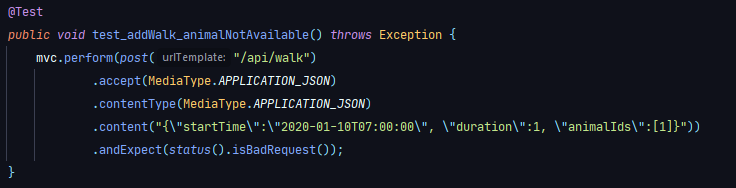
\includegraphics[width=\linewidth]{slike/Testovi-10.png}
		\centering
		\caption{Testiranje šetnje za koju životinja nije dostupna}
		\label{fig:testovi10}
	\end{figure}

	\eject

	\noindent Na API poziv "/api/walk/animals" šaljemo podatke o željenom početku šetnje, trajanju i odabranu udrugu. Cilj nam je provjeriti dostupnost životinje u navedenom terminu. Očekivani rezultat je statusni kod 200.

	\begin{figure}[H]
		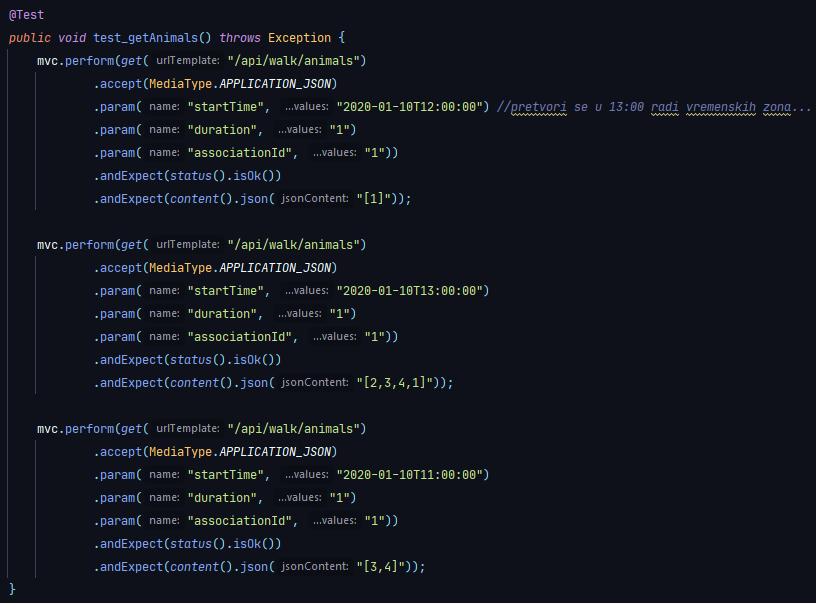
\includegraphics[width=\linewidth]{slike/Testovi-11.png}
		\centering
		\caption{Testiranje dostupnosti životinja}
		\label{fig:testovi11}
	\end{figure}

	\eject

	\noindent Slijede rezultati navedenih testova.

	\begin{figure}[H]
		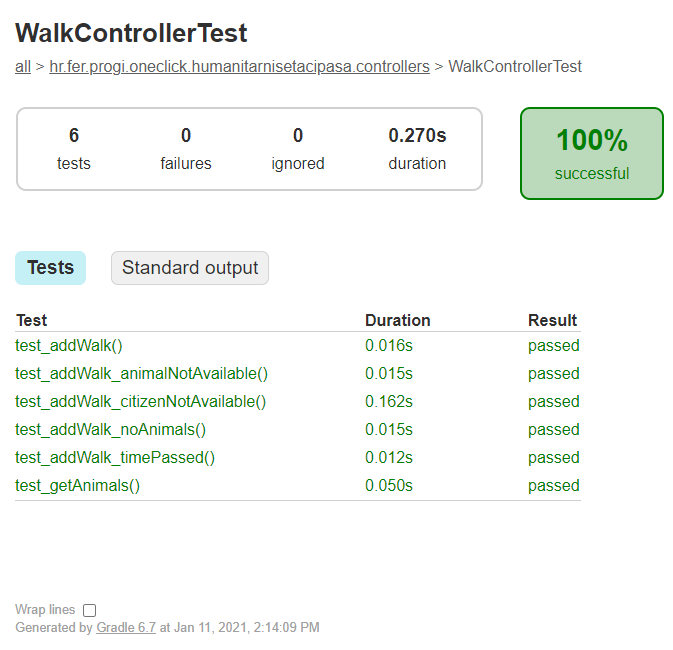
\includegraphics[width=\linewidth]{slike/Testovi-16.png}
		\centering
		\caption{Rezultati testiranja WalkControllera}
		\label{fig:testovi16}
	\end{figure}

	\eject
	
	\noindent Postavljeni su podaci za jednu udrugu. 
	
	\begin{figure}[H]
		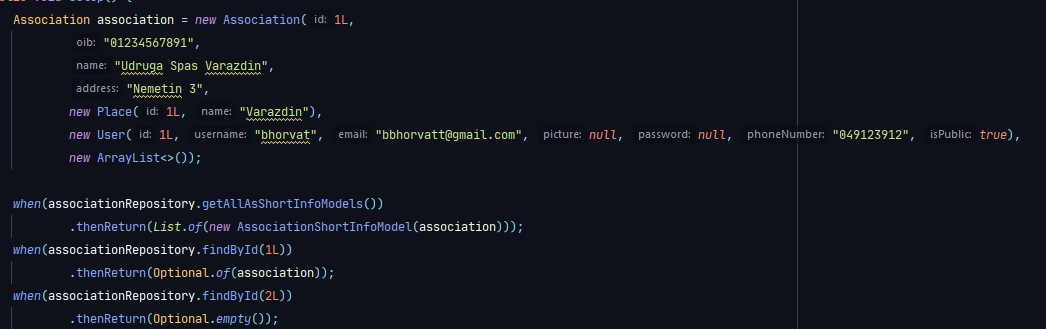
\includegraphics[width=\linewidth]{slike/Testovi-12.png}
		\centering
		\caption{Postavljanje testnih podataka za testiranje AssociationControllera}
		\label{fig:testovi12}
	\end{figure}


	\noindent Na API poziv "/api/association" šaljemo zahtjev za  dohvat svih udruga. Očekivani rezultat je statusni kod 200.

	\begin{figure}[H]
		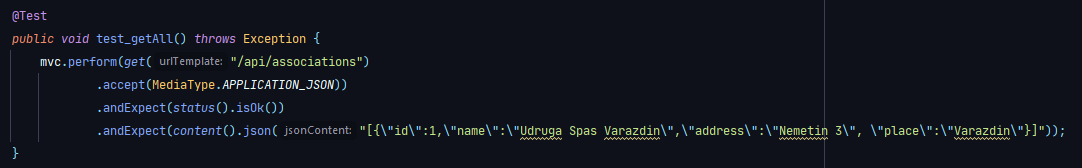
\includegraphics[width=\linewidth]{slike/Testovi-13.png}
		\centering
		\caption{Testiranje dohvata svih udruga}
		\label{fig:testovi13}
	\end{figure}

	\noindent  Na API poziv "/api/association/1" šaljemo zahtjev za dohvat udruge sa šifrom 1. Očekivani rezultat je statusni kod 200.

	\begin{figure}[H]
		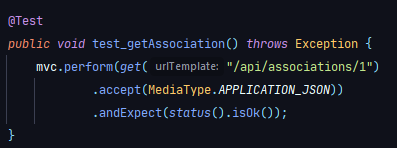
\includegraphics[width=\linewidth]{slike/Testovi-14.png}
		\centering
		\caption{Testiranje dohvata odabrane udruge}
		\label{fig:testovi14}
	\end{figure}

	\noindent Na API poziv "/api/association/2" šaljemo zahtjev za dohvat udruge sa šifrom 2. Očekivani rezultat je statusni kod 400.

	\begin{figure}[H]
		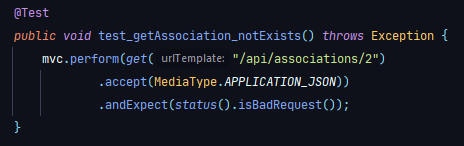
\includegraphics[width=\linewidth]{slike/Testovi-15.png}
		\centering
		\caption{Testiranje dohvata udruge koja ne postoji}
		\label{fig:testovi15}
	\end{figure}

	\eject

	\noindent Slijede rezultati navedenih testova.

	\begin{figure}[H]
		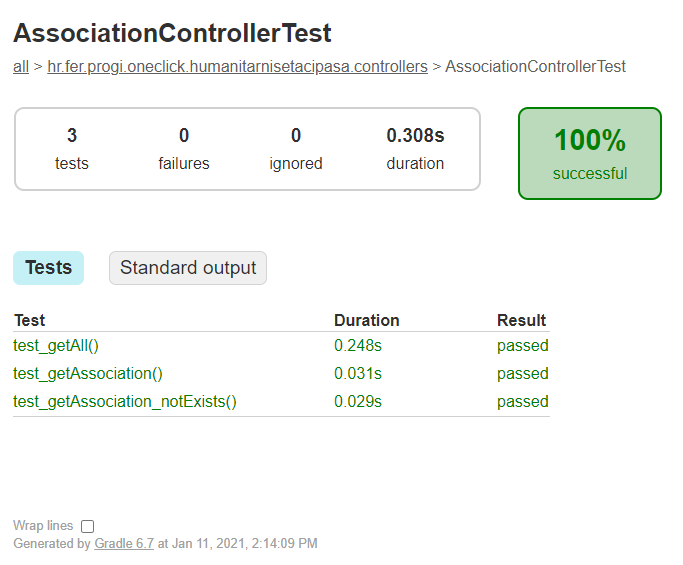
\includegraphics[width=\linewidth]{slike/Testovi-17.png}
		\centering
		\caption{Rezultati testiranja AssociationControllera}
		\label{fig:testovi17}
	\end{figure}
	
	\eject

	\subsection{Ispitivanje sustava}
	
	\noindent Ulaz za prvi test je nevaljano korisničko ime i lozinka. Očekivani rezultat je prikazivanje poruke "Pogrešni podaci za prijavu!".
	
	\begin{figure}[H]
		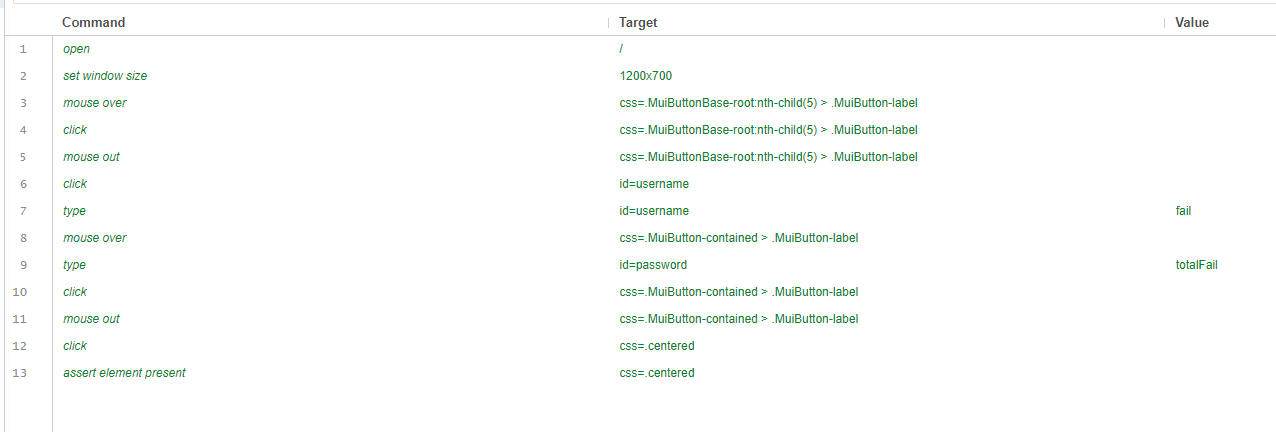
\includegraphics[width=\linewidth]{slike/front-testovi-1.png}
		\centering
		\caption{Koraci prvog testa}
		\label{fig:fronttestovi1}
	\end{figure}
	
	\noindent \newline Rezultat prvog testa je prikaz poruke "Pogrešni podaci za prijavu!".

	\begin{figure}[H]
		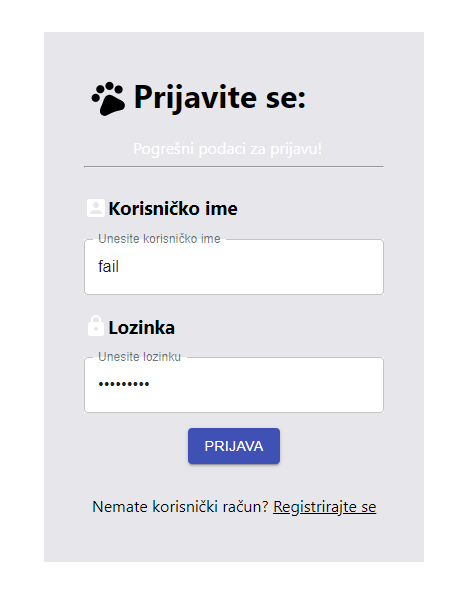
\includegraphics [width=0.50\linewidth]{slike/front-testovi-2.png}
		\centering
		\caption{Rezultat prvog testa}
		\label{fig:fronttestovi2}
	\end{figure}

	\eject

	\noindent Ulaz za drugi test su ispravni podaci. Očekivani rezultat je prijava u sustav.

	\begin{figure}[H]
		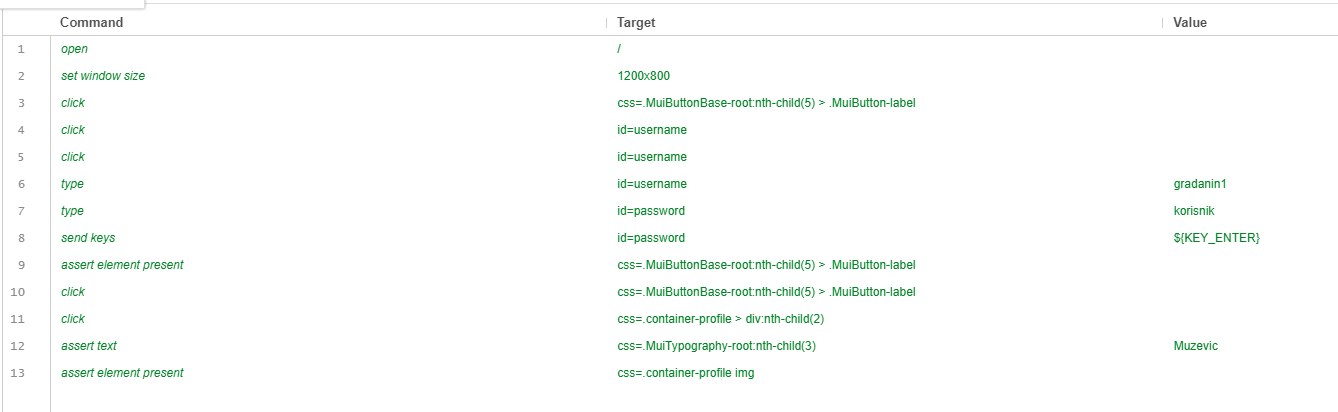
\includegraphics[width=\linewidth]{slike/front-testovi-3.png}
		\centering
		\caption{Koraci drugog testa}
		\label{fig:fronttestovi3}
	\end{figure}

	\noindent \newline Rezultat drugog testa je prijava u sustav s danim korisničkim imenom i lozinkom.

	\begin{figure}[H]
		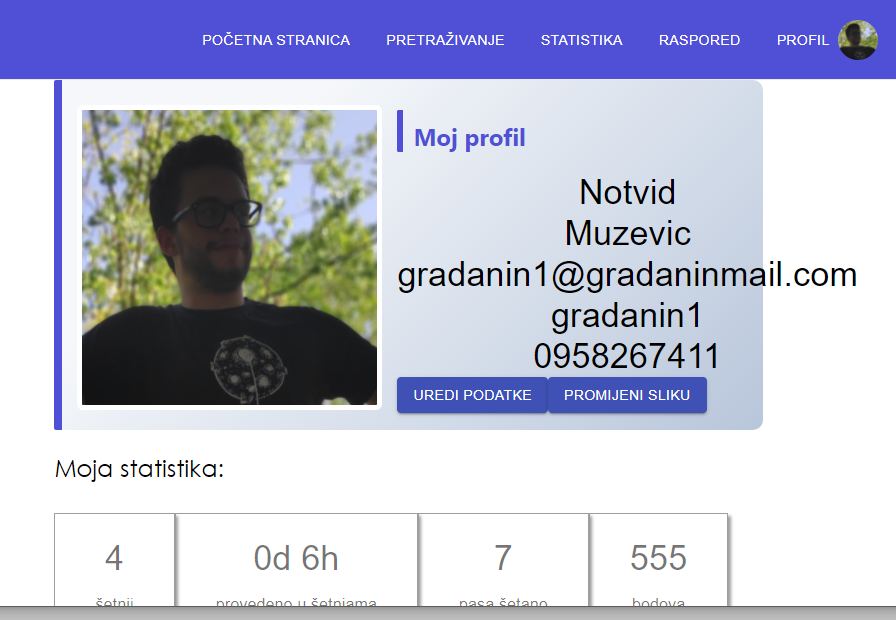
\includegraphics[width=0.8\linewidth]{slike/front-testovi-4.png}
		\centering
		\caption{Rezultat drugog testa}
		\label{fig:fronttestovi4}
	\end{figure}

	\eject

	\noindent Ulaz za treći test su podaci za registraciju. Očekivani rezultat je registracija u sustav.

	\begin{figure}[H]
		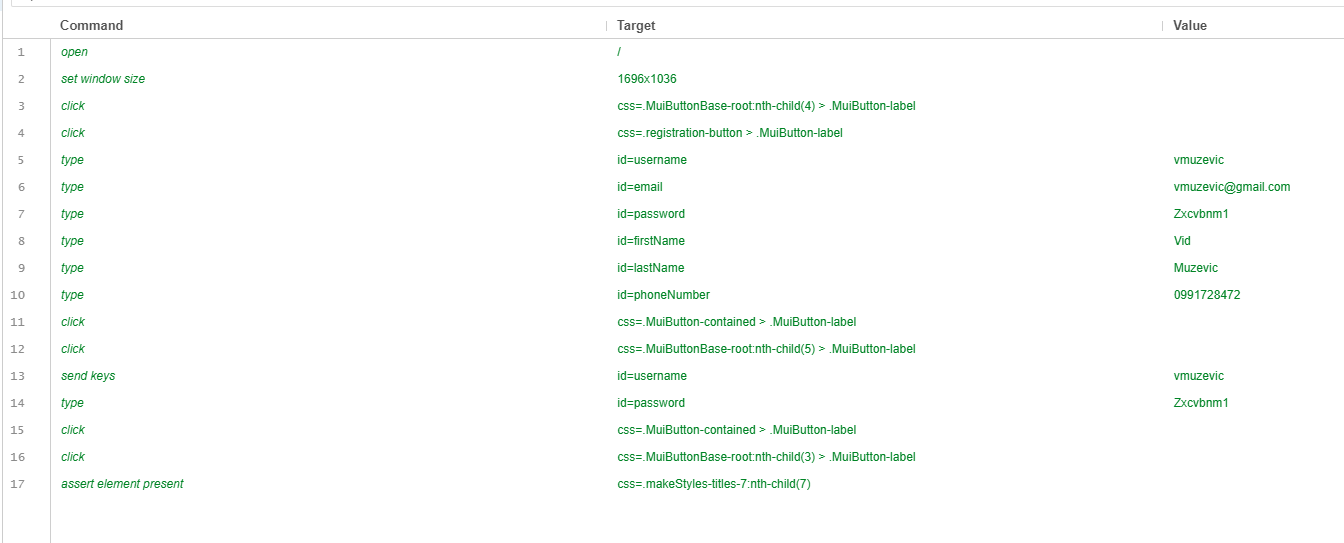
\includegraphics[width=\linewidth]{slike/front-testovi-5.png}
		\centering
		\caption{Koraci trećeg testa}
		\label{fig:fronttestovi5}
	\end{figure}

	\noindent \newline Rezultat trećeg testa je registracija u sustav s danim podacima.

	\begin{figure}[H]
		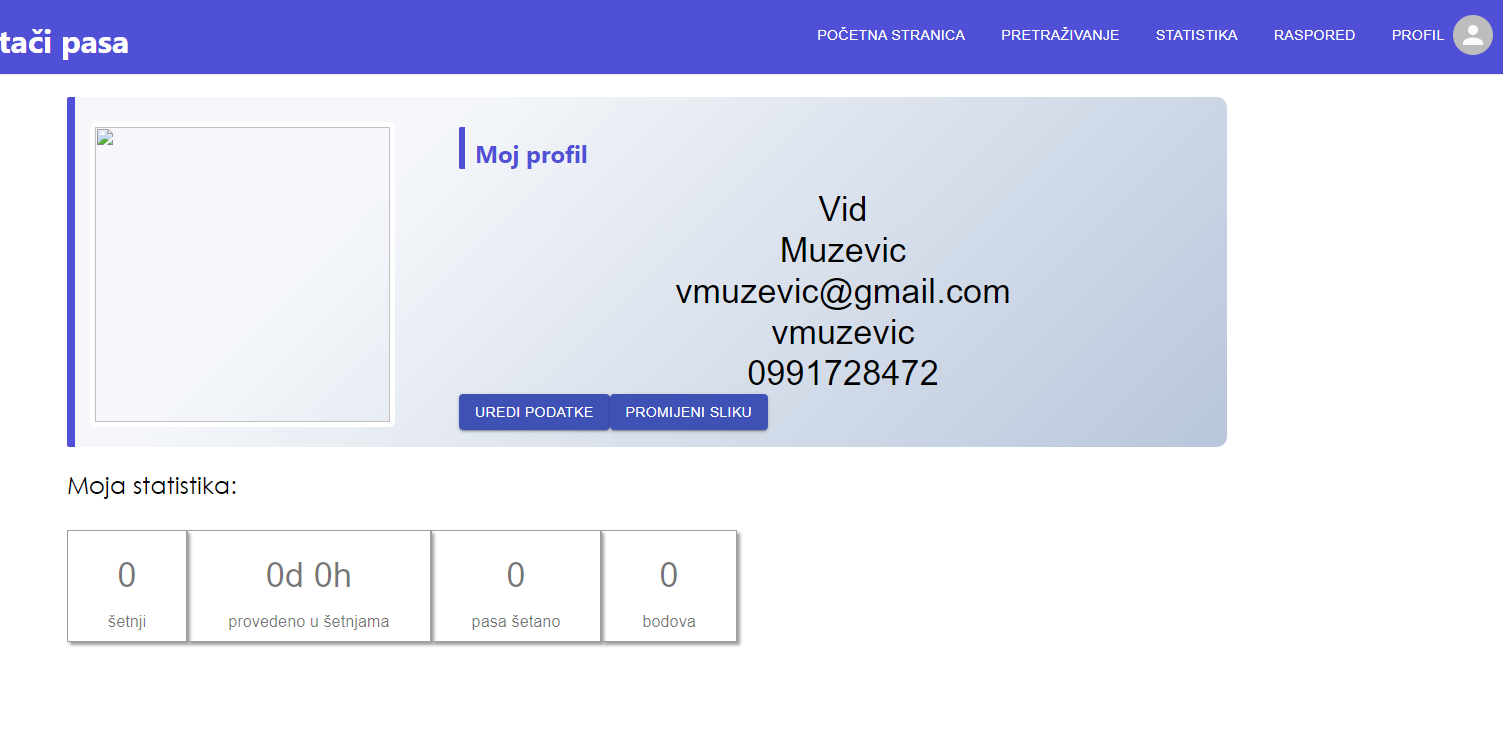
\includegraphics[width=0.9\linewidth]{slike/front-testovi-6.png}
		\centering
		\caption{Rezultat trećeg testa}
		\label{fig:fronttestovi6}
	\end{figure}

	\eject

	\noindent Ulaz za četvrti test su podaci koje želimo urediti, tj. promijeniti njihovu vrijednost. Očekivani rezultat su promijenjeni podaci na stranici profila.

	\begin{figure}[H]
		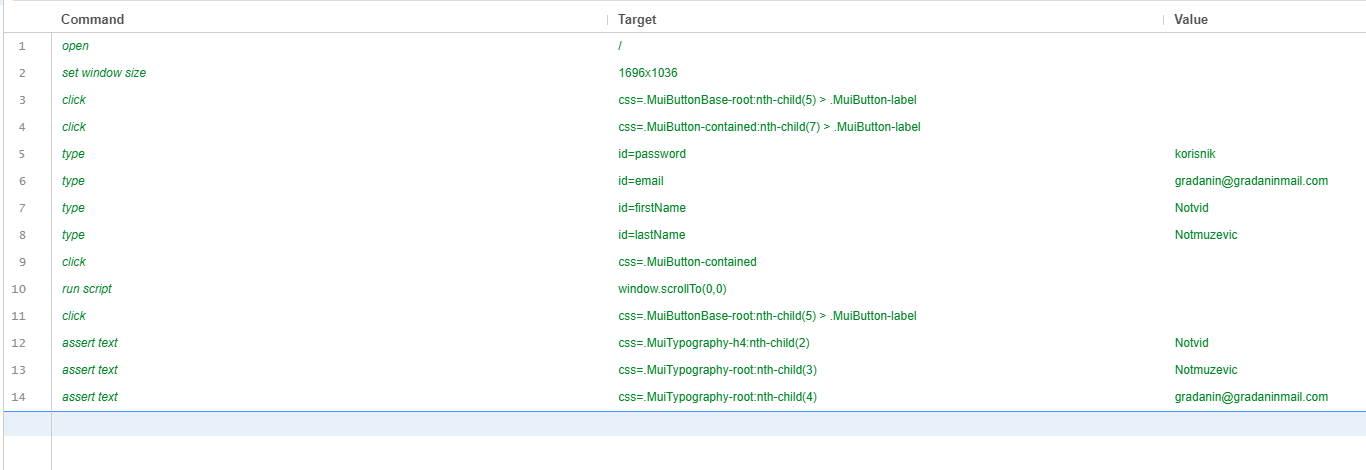
\includegraphics[width=\linewidth]{slike/front-testovi-7.png}
		\centering
		\caption{Koraci četvrtog testa}
		\label{fig:fronttestovi7}
	\end{figure}

	\noindent \newline Rezultat četvrtog testa su promijenjeni podaci na stranici profila.

	\begin{figure}[H]
		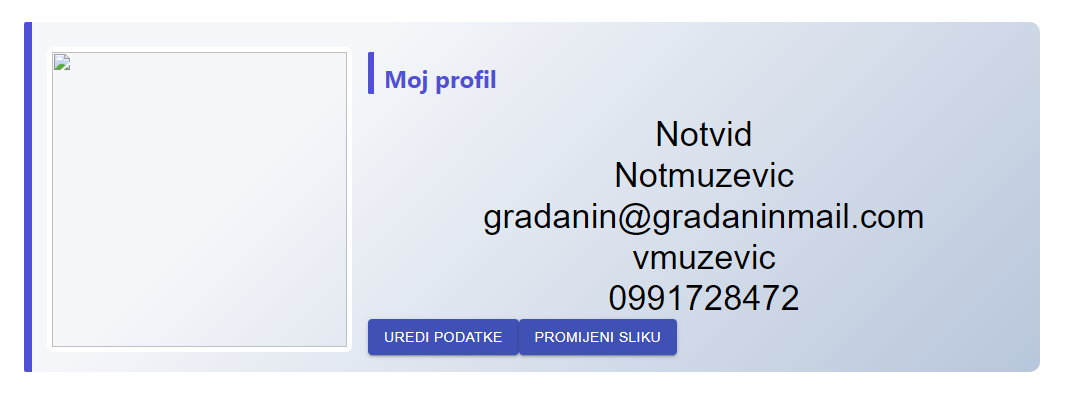
\includegraphics[width=\linewidth]{slike/front-testovi-8.png}
		\centering
		\caption{Rezultat četvrtog testa}
		\label{fig:fronttestovi8}
	\end{figure}

	\eject

	\noindent Ulaz petog testa su podaci za prijavu šetnje, tj. datum, vrijeme početka i trajanje šetnje. U testu se odabir datuma i vremena šetnje provodi klikanjem na elemente za odabir datuma i vremena. Očekivani rezultat je prijava šetnje.

	\begin{figure}[H]
		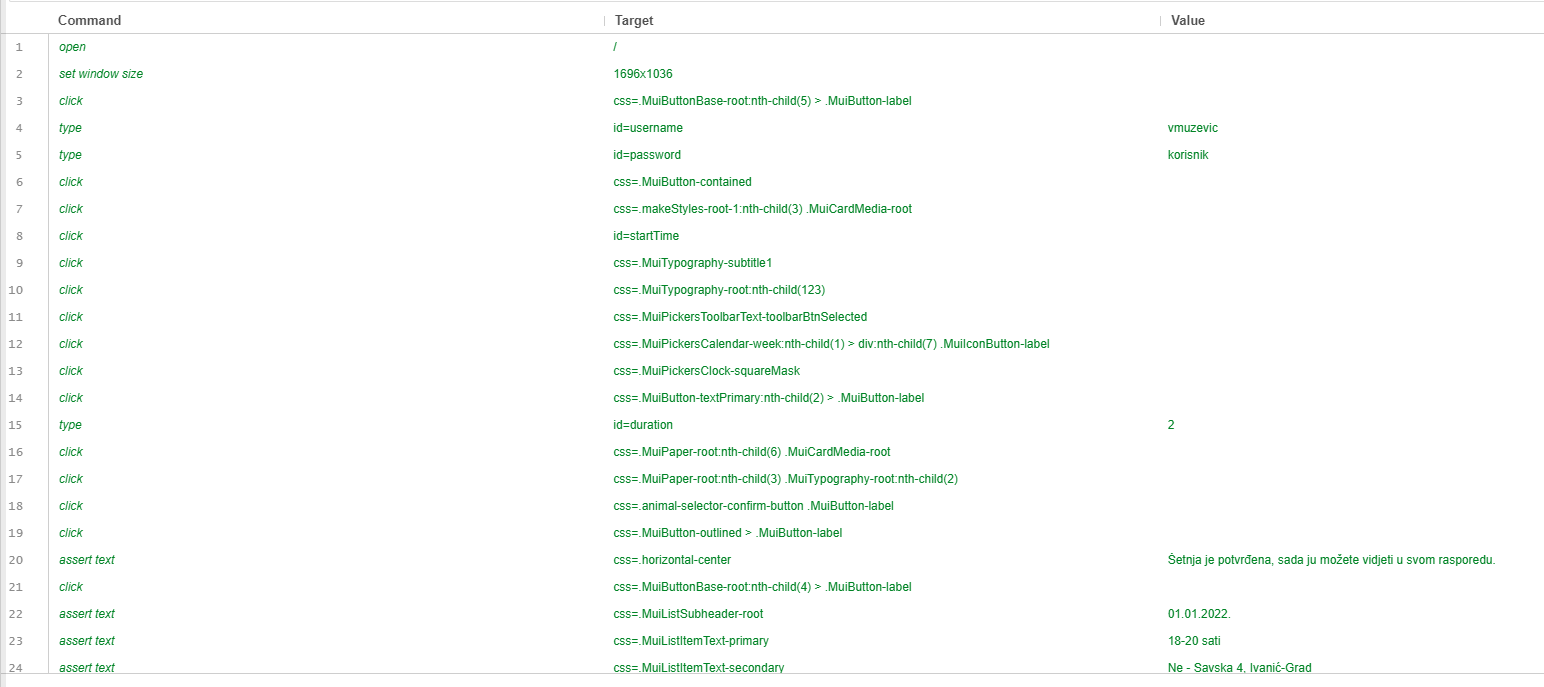
\includegraphics[width=\linewidth]{slike/front-testovi-9.png}
		\centering
		\caption{Koraci petog testa}
		\label{fig:fronttestovi9}
	\end{figure}

	\noindent \newline Rezultat petog testa je prijavljena šetnja koja se može vidjeti u rasporedu.

	\begin{figure}[H]
		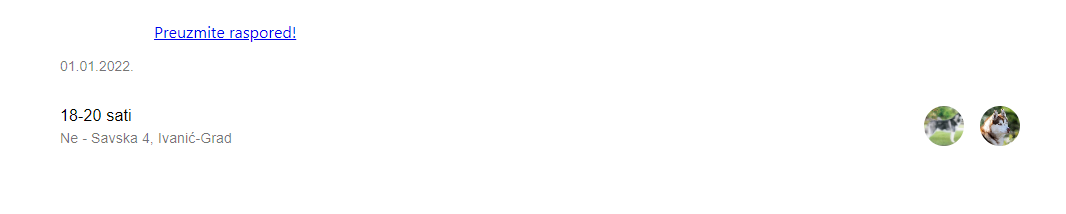
\includegraphics[width=\linewidth]{slike/front-testovi-10.png}
		\centering
		\caption{Rezultat petog testa}
		\label{fig:fronttestovi10}
	\end{figure}

	\eject

	\noindent Ulaz u šesti test su podaci o novoj životinji koju se želi dodati na stranicu udruge. Pretpostavka je da smo prijavljeni u sustav kao udruga. Očekivani rezultat je dodana životinja na stranicu udruge.

	\begin{figure}[H]
		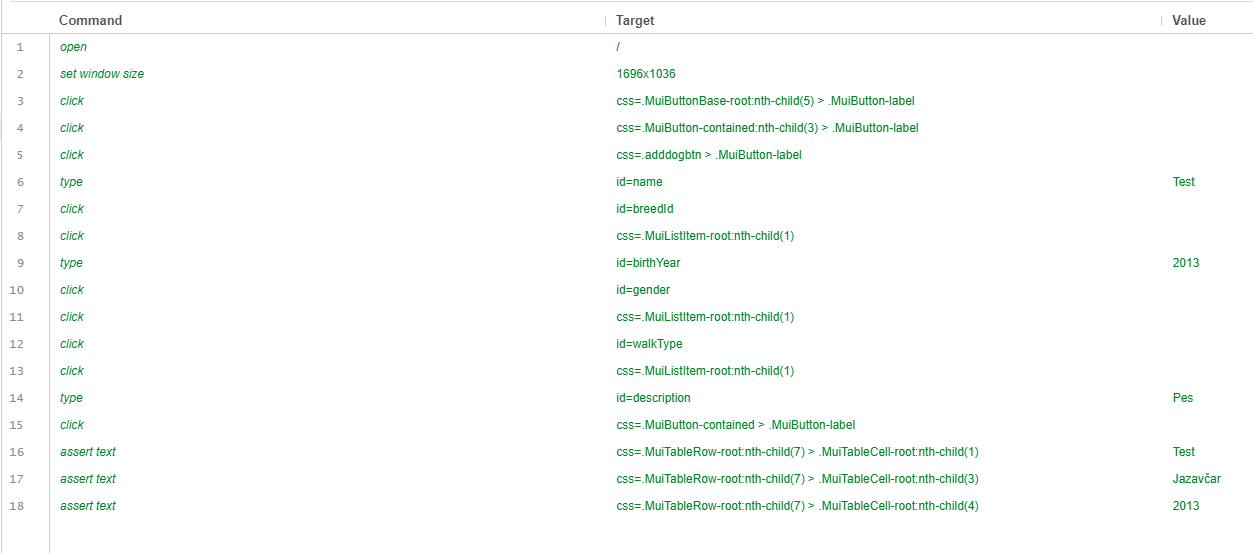
\includegraphics[width=\linewidth]{slike/front-testovi-11.png}
		\centering
		\caption{Koraci šestog testa}
		\label{fig:fronttestovi11}
	\end{figure}

	\noindent \newline Rezultat šestog testa je dodana životinja na stranicu udruge.

	\begin{figure}[H]
		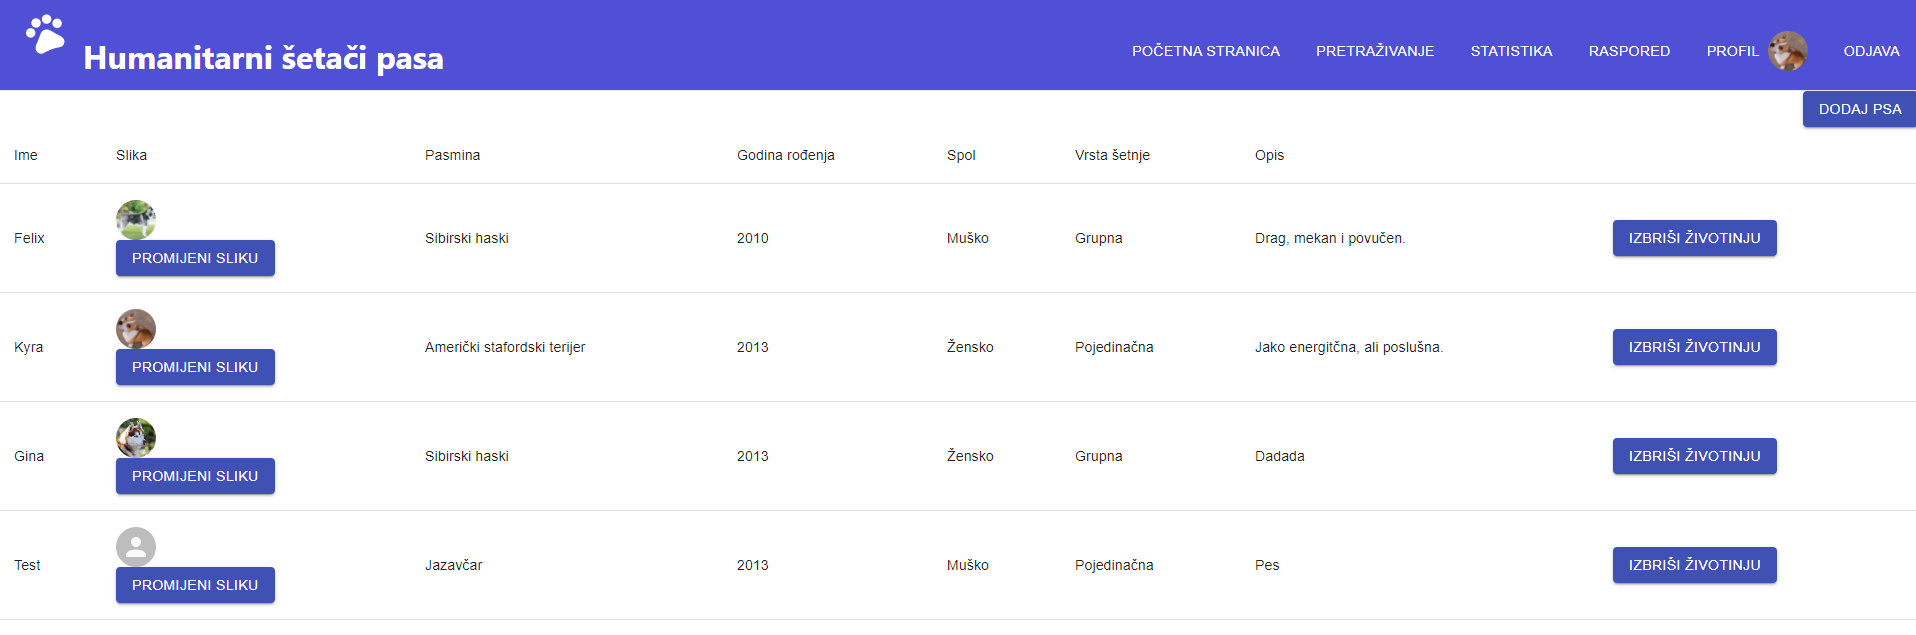
\includegraphics[width=\linewidth]{slike/front-testovi-12.png}
		\centering
		\caption{Rezultat šestog testa}
		\label{fig:fronttestovi12}
	\end{figure}

	\eject

	\noindent Ulaz sedmog testa je klik na gumb "Izbriši životinju". Očekivani rezultat je brisanje životinje dodane u prethodnom testu.

	\begin{figure}[H]
		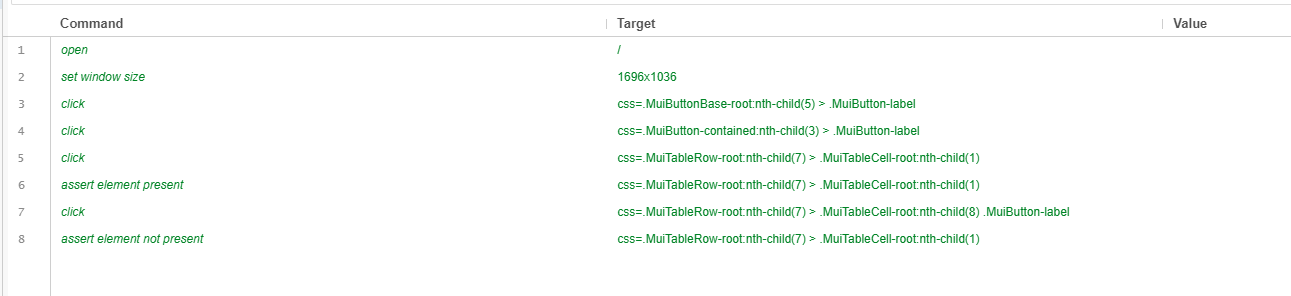
\includegraphics[width=\linewidth]{slike/front-testovi-13.png}
		\centering
		\caption{Koraci sedmog testa}
		\label{fig:fronttestovi13}
	\end{figure}

	\noindent \newline Rezultat sedmog testa je brisanje životinje dodane u prethodnom testu.

	\begin{figure}[H]
		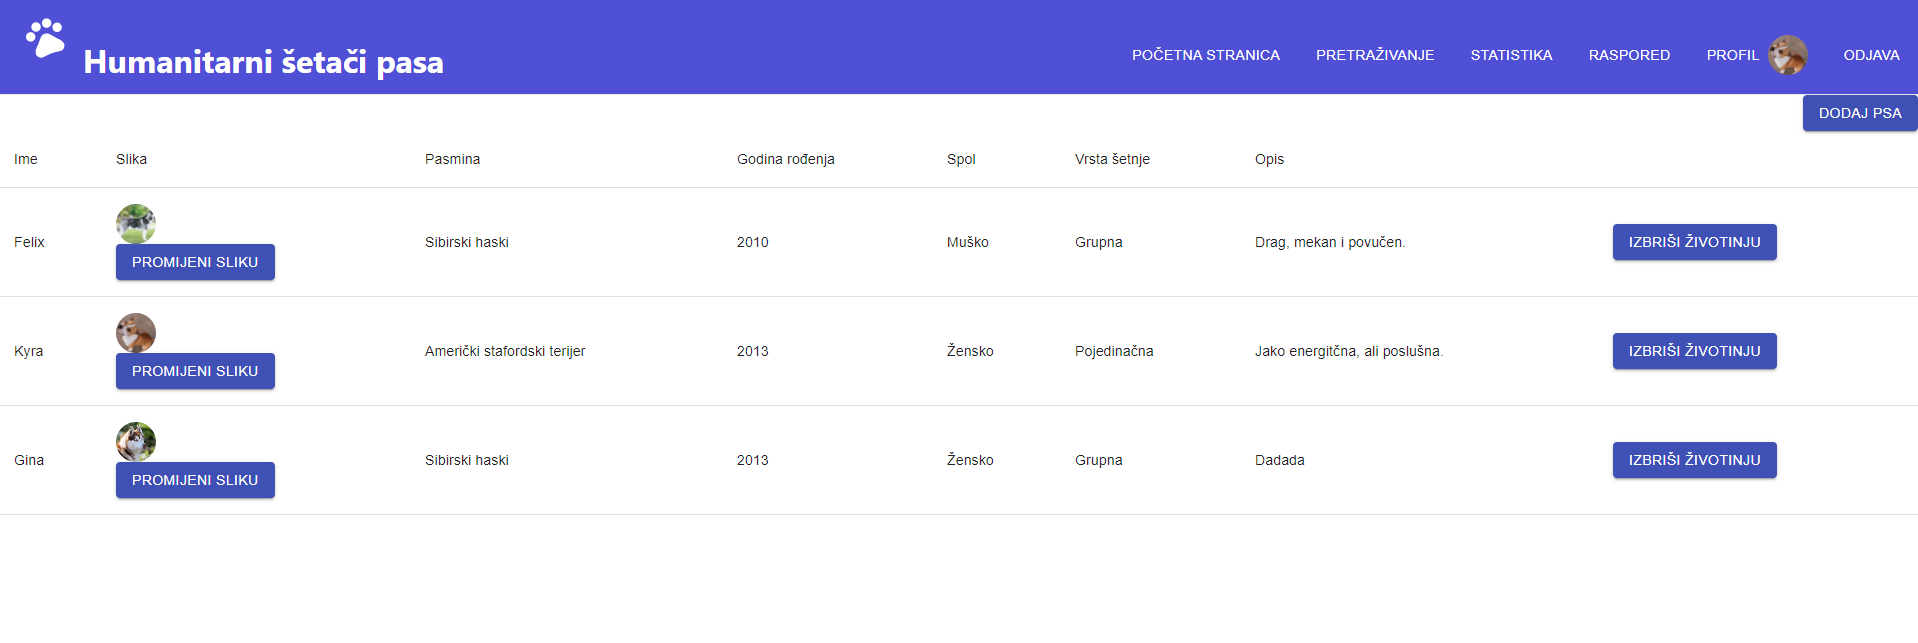
\includegraphics[width=\linewidth]{slike/front-testovi-14.png}
		\centering
		\caption{Rezultat sedmog testa}
		\label{fig:fronttestovi14}
	\end{figure}
	
	\eject
	
	\section{Dijagram razmještaja}
	\begin{figure}[H]
		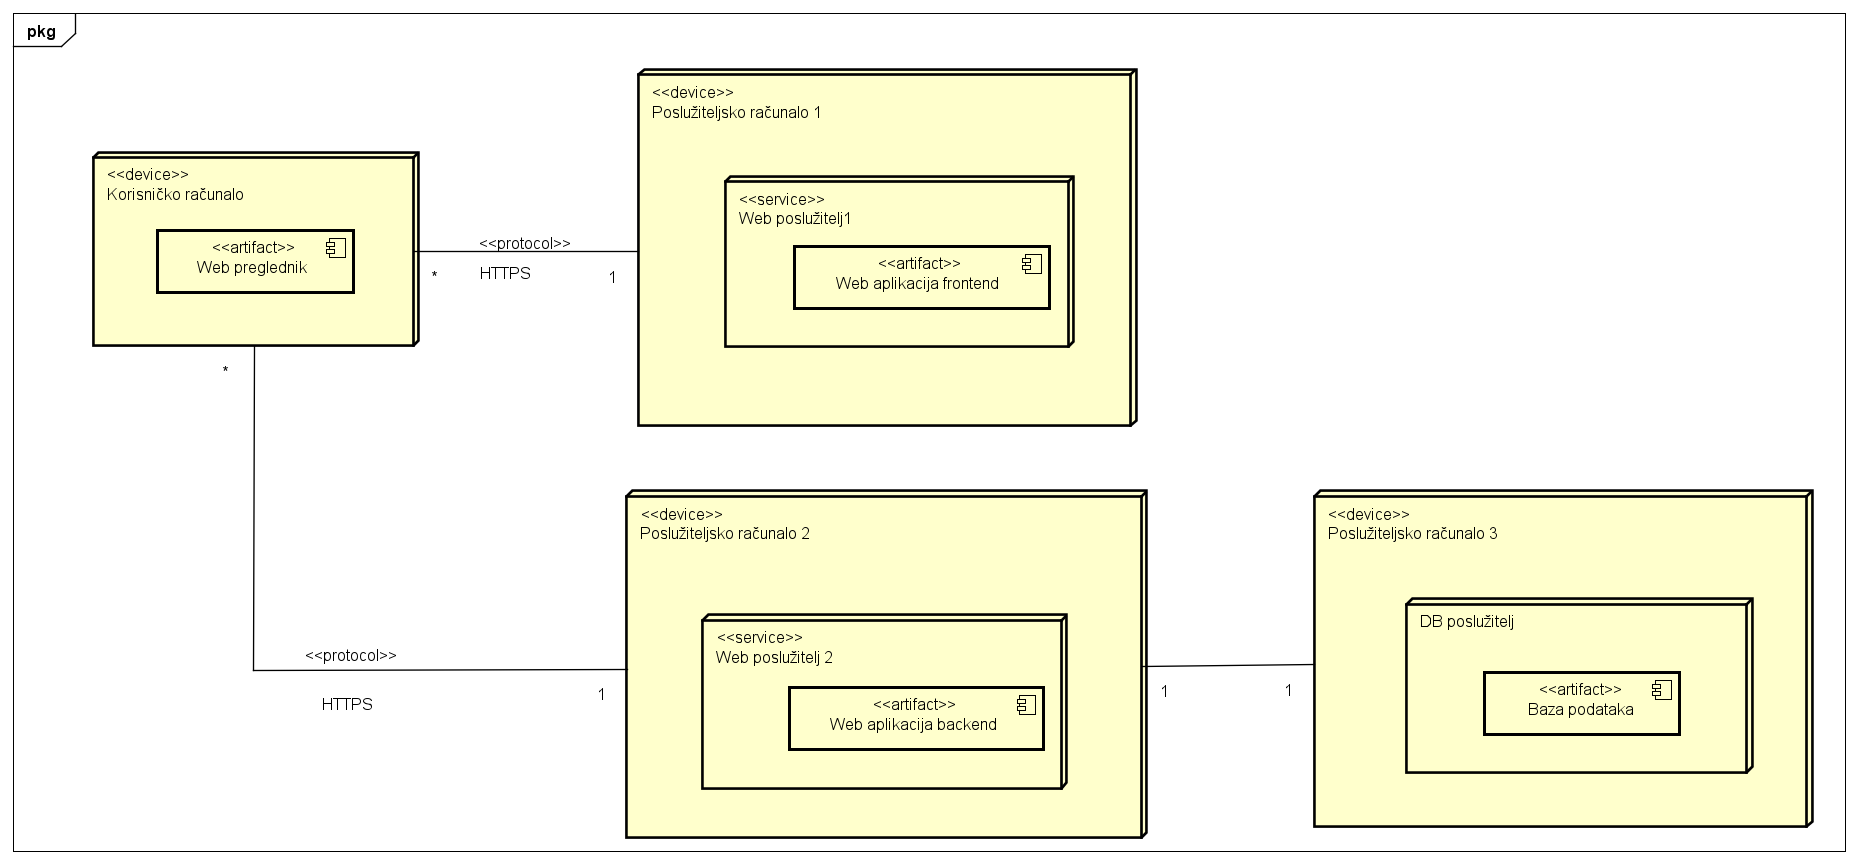
\includegraphics[width=\linewidth]{slike/DeploymentDiagram0.png}
		\centering
		\caption{Dijagram razmještaja}
		\label{fig:dijagramrazmještaja}
	\end{figure}
\eject
\section{Upute za puštanje u pogon}

Za puštanje aplikacije u pogon, ponajprije treba napraviti račun na besplatnoj usluzi za deploy aplikacija - Heroku.
Nakon toga treba napraviti nove projekte i dodati dodatke u same projekte. Odlučili smo se napraviti dva nova projekta, jedan za backend te jedan za frontend.
Kod deploya za backend potrebno je povezati bazu podataka i instalirati ju kao dodatak projektu.
\begin{figure}[H]
	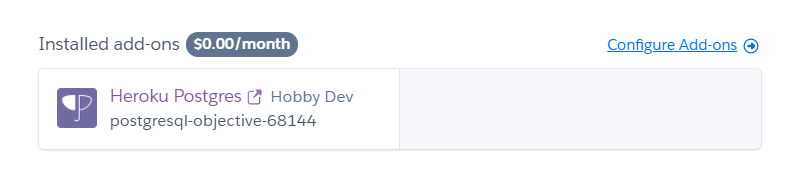
\includegraphics[width=\linewidth]{slike/heroku-backend.png}
	\centering
	\caption{Povezivanje baze podataka na backend projekt}
	\label{fig:postgresqlbackend}
\end{figure}
Za bazu podataka odlučili smo koristiti PostgreSQL koju je pritom bilo potrebno instalirati na vlastiti operacijski sustav. Nakon dodavanja baze na backend projekt bilo je potrebno tu istu bazu povezati sa našom aplikacijom. Kako bismo to učinili, na vlastitom backend projektu morali smo promijeniti application.properties datoteku. U toj datoteci morali smo promijeniti korisničko ime, lozinku i poveznicu na bazu podataka. Nakon toga baza je bila spremna za punjenje podatcima. Uz to smo dodali i datoteku application-local.properties kako bismo samu aplikaciju mogli pokretati i preko vlastitog localhosta. 
Za izradu frontend dijela projekta koristili smo React, stoga je u sam projekt bilo potrebno dodati buildpack kako bi se instalirale ovisnosti s obzirom na React.
\begin{figure}[H]
	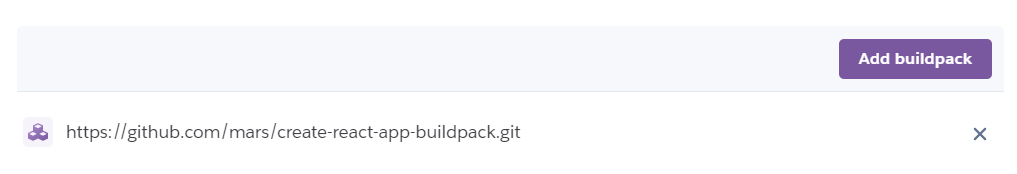
\includegraphics[width=\linewidth]{slike/heroku-frontend.png}
	\centering
	\caption{Povezivanje Reacta na frontend projekt}
	\label{fig:reactfrontend}
\end{figure}
Nakon dodavanja backenda i frontenda dodali smo još i pipelineove koji su nam olakšavali deployment na Heroku. Pipelineovi su se pokretali izvršavanjem .gitlab-ci.yml datoteke u samom korijenu dokumenta. Za njihovo izvršavanje bilo je potrebno postaviti varijable na gitlabu pomoću kojih smo pristupali backendu i frontendu na Heroku.
\begin{figure}[H]
	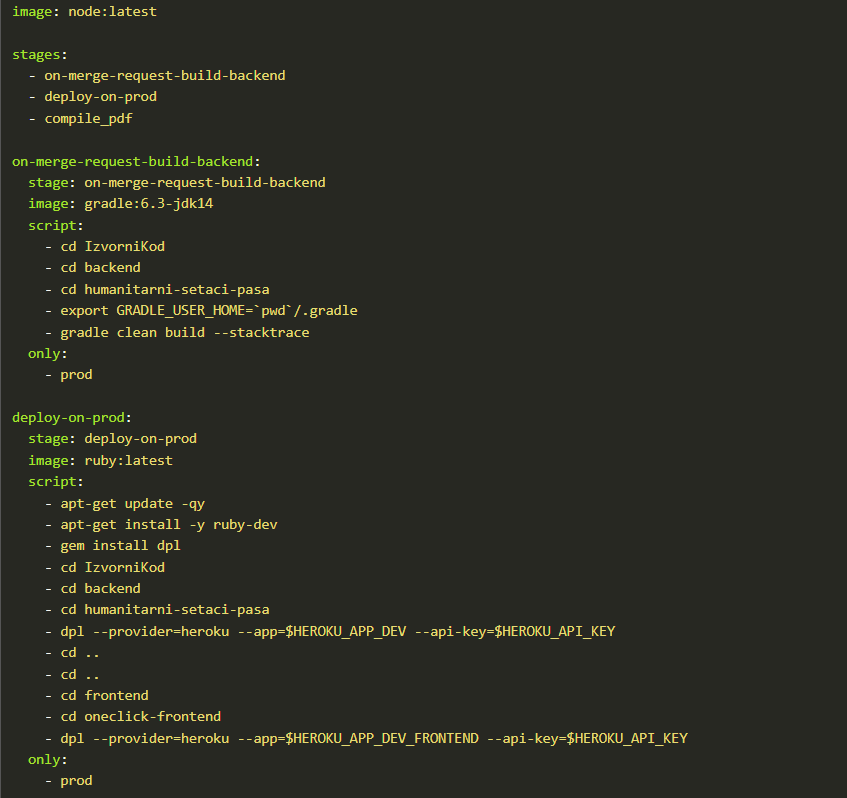
\includegraphics[width=\linewidth]{slike/heroku-cicd.png}
	\centering
	\caption{Datoteka .gitlab-ci.yml korištena kod deploymenta}
	\label{fig:gitlabci}
\end{figure}
Uz pipelineove za deploy dodali smo i jedan za generiranje pdf dokumenta koji je latex dokument pretvorio u pdf koji smo mogli preuzeti. Na taj smo način bili sigurni da se slučajno nije dogodila pogreška prilikom pisanja dokumentacije.
Svi ovi pipelineovi omogućili su nam da prilikom mergea na granu koju smo zadali provjerimo je li došlo do pogreške te zatim aplikaciju uspješno deployamo na Heroku.
\begin{figure}[H]
	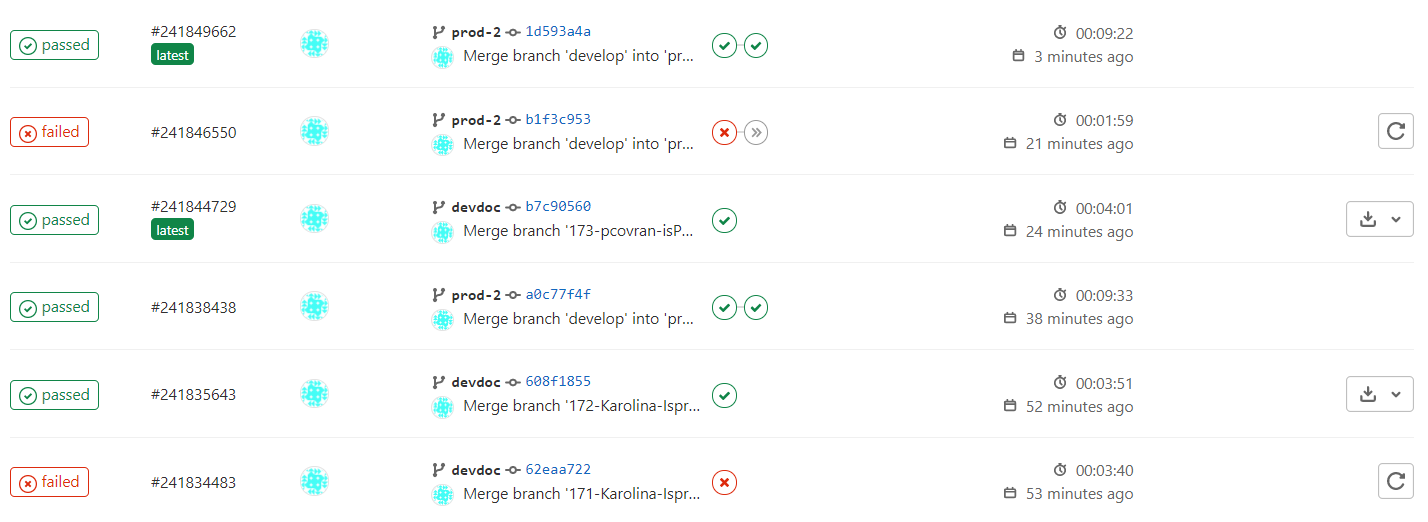
\includegraphics[width=\linewidth]{slike/heroku-pipelines.png}
	\centering
	\caption{Primjer pipelineova}
	\label{fig:pipelines}
\end{figure}
	\chapter{Zaključak i budući rad}
		
		 Naš zadatak bio je razviti web aplikaciju (prilagođenu za mobilne uređaje) za humanitarno šetanje pasa koja omogućuje udrugama za životinje da ponude nezbrinute pse za šetnju, a građanima da dobrovoljno šetaju pse uz mogućnost pristupa vlastitom rasporedu šetnji i statistici šetača. Nakon 16 tjedana timskog rada, ostvarili smo zadani cilj, a taj proces odvijao se u dvije faze.
		
		 Prva faza projekta započela je okupljanjem razvojnog tima, dodjelom projektnog zadatka, upoznavanjem sa zahtjevima te njihovim definiranjem i dokumentiranjem. Detaljno definiranje zahtjeva na početku rada na projektu pokazalo se kao velika prednost pri implementaciji te omogućilo lakše planiranje rada i podjelu posla. Definiranje dijagrama obrazaca uporabe, sekvencijskih dijagrama, modela baze podataka i dijagrama razreda pružili su nam jasnu i jednoznačnu ideju ostvarenja funkcionalnosti naše aplikacije.
		 
		 Druga faza projekta velikim dijelom sastojala se od kodiranja i implementacije traženih funkcionalnosti. Članovi su si izabrali zadatke prema osobnim predznanjima i interesima, no svi su se barem s nekom od korištenih tehnologija susreli po prvi puta, što ih je prisililo i potaknulo na samostalno učenje i napredak te međusobno dijeljenje znanja. Dobro definirani zahtjevi na početku spriječili su moguće nesporazume koji u kasnijom fazi implementacije mogu biti vrlo problematični i vremenski skupi. Također, bilo je potrebno dokumentirati dijagrame stanja, aktivnosti, komponenti i razmještaja te napisati upute za korištenje razvijene aplikacije.
		 
		 Za vrijeme rada na projektu, članovi su komunicirali putem Whatsappa, na kojem su dijelili najvažnije informacije i dogovarali termine sastanaka, te putem Discorda, gdje su održavali sastanke, pratili dotadašnji napredak i razrađivali daljnje korake rada. Komunikacija članova tima bila je vrlo kvalitetna te je vladala pozitivna radna atmosfera.
		 
		 Sudjelovanje u ovom projektu bilo je vrlo ugodno i poučno iskustvo te nas je kao buduće inženjere obogatilo ne samo tehničkim znanjima, nego i boljim komunikacijskim vještinama i iskustvom rada u grupi. Iako bi prethodno iskustvo rada na sličnim projektima uvelike olakšalo i ubrzalo razvoj naše aplikacije te konačni proizvod zasigurno učinilo kvalitetnijim, zadovoljni smo postignutim rezultatima i vjerujemo da ćemo mnoga stečena znanja ponijeti sa sobom u buduće projekte koji nas čekaju kroz našu karijeru.
	\chapter*{Popis literature}
		\addcontentsline{toc}{chapter}{Popis literature}
	 	
		
		
		\begin{enumerate}
			
			
			\item  Programsko inženjerstvo, FER ZEMRIS, \url{http://www.fer.hr/predmet/proinz}
			
			\item  I. Sommerville, "Software engineering", 8th ed, Addison Wesley, 2007.
			
			\item  T.C.Lethbridge, R.Langaniere, "Object-Oriented Software Engineering", 2nd ed. McGraw-Hill, 2005.
			
			\item  I. Marsic, Software engineering book``, Department of Electrical and Computer Engineering, Rutgers University, \url{http://www.ece.rutgers.edu/~marsic/books/SE}
			
			\item  The Unified Modeling Language, \url{https://www.uml-diagrams.org/}
			
			\item  Astah Community, \url{http://astah.net/editions/uml-new}
		\end{enumerate}
		
		 
	
	
	\begingroup
	\renewcommand*\listfigurename{Indeks slika i dijagrama}
	%\renewcommand*\listtablename{Indeks tablica}
	%\let\clearpage\relax
	\listoffigures
	%\vspace{10mm}
	%\listoftables
	\endgroup
	\addcontentsline{toc}{chapter}{Indeks slika i dijagrama}


	
	\eject 
		
	\chapter*{Dodatak: Prikaz aktivnosti grupe}
		\addcontentsline{toc}{chapter}{Dodatak: Prikaz aktivnosti grupe}
		
		\section*{Dnevnik sastajanja}
		
		
		\begin{packed_enum}
			\item  sastanak
			
			\item[] \begin{packed_item}
				\item Datum: 7. listopada 2020.
				\item Prisustvovali: Benjamin Horvat, Iva Zekić, Petar Čovran, Mihael Rodek, Dora Doljanin, Vid Mužević, Karolina Mirković
				\item Teme sastanka:
				\begin{packed_item}
					\item  upoznavanje članova
					\item  dogovor o komuniciranju putem Discord servera
					\item  početna riječ o načelima vođenja projekta koji će se primijeniti
					\item  komentiranje zadanog zadatka
				\end{packed_item}
			\end{packed_item}
			
			\item  sastanak
			\item[] \begin{packed_item}
				\item Datum: 15. listopada 2020.
				\item Prisustvovali: Benjamin Horvat, Iva Zekić, Petar Čovran, Mihael Rodek, Dora Doljanin, Vid Mužević, Karolina Mirković
				\item Teme sastanka:
				\begin{packed_item}
					\item  instalacija Git-a, TeXLive i TeXStudio kod svih članova grupe
					\item  upoznavanje s Git-om
					\item  upoznavanje s GitLab-om
					\item  dogovaranje načina korištenja branchova, issuea i merge requestova
					\item  početak pisanja funkcionalnih zahtjeva
					\item  početak razrade strukture baze podataka 
				\end{packed_item}
				\item Zadaci do idućeg sastanka:
				\begin{packed_item}
					\item  provjera funkcionalnih zahtjeva i sastavljanje pitanja vezano za njih
				\end{packed_item}
			\end{packed_item}
		
		\item  sastanak
		
		\item[] \begin{packed_item}
			\item Datum: 19. listopada 2020.
			\item Prisustvovali: Benjamin Horvat, Petar Čovran, Mihael Rodek, Dora Doljanin, Vid Mužević, Karolina Mirković
			\item Teme sastanka:
			\begin{packed_item}
				\item  dovršavanje funkcionalnih zahtjeva
				\item  raspisivanje svih use caseova
			\end{packed_item}
			\item Zadaci do idućeg sastanka:
			\begin{packed_item}
				\item  pregled raspisanih use caseova
			\end{packed_item}
		\end{packed_item}
	
		\item  sastanak
		
		\item[] \begin{packed_item}
			\item Datum: 22. listopada 2020.
			\item Prisustvovali: Benjamin Horvat, Iva Zekić, Petar Čovran, Mihael Rodek, Dora Doljanin, Vid Mužević, Karolina Mirković
			\item Teme sastanka:
			\begin{packed_item}
				\item  stvaranje UML dijagrama
				\item  podjela issuea za upisivanje dokumentacije u LaTeX
			\end{packed_item}
			\item Zadaci do idućeg sastanka:
			\begin{packed_item}
				\item  riješiti issuee na GitLabu
			\end{packed_item}
		\end{packed_item}
	
		\item  sastanak
		
		\item[] \begin{packed_item}
			\item Datum: 27. listopada 2020.
			\item Prisustvovali: Benjamin Horvat, Petar Čovran, Mihael Rodek, Dora Doljanin, Vid Mužević, Karolina Mirković
			\item Teme sastanka:
			\begin{packed_item}
				\item  stvaranje frontend React projekta sa TypeScriptom
				\item  stvaranje backend Java Spring Boot projekta
				\item  stvaranje sekvencijskih dijagrama
				\item  stvaranje ER dijagrama baze podataka
			\end{packed_item}
			\item Zadaci do idućeg sastanka:
			\begin{packed_item}
				\item  raspisati issuee 
				\item  dovršiti ER i sekvencijske dijagrame
			\end{packed_item}
		\end{packed_item}
	
		\item  sastanak
		
		\item[] \begin{packed_item}
			\item Datum: 28. listopada 2020.
			\item Prisustvovali: Benjamin Horvat, Iva Zekić, Petar Čovran, Mihael Rodek, Dora Doljanin, Vid Mužević, Karolina Mirković
			\item Teme sastanka:
			\begin{packed_item}
				\item  dovršavanje sekvencijskih dijagrama
				\item  dovršavanje ER dijagrama
			\end{packed_item}
			\item Zadaci do idućeg sastanka:
			\begin{packed_item}
				\item  raspisati issuee 
			\end{packed_item}
		\end{packed_item}
		
		\item sastanak
		
		\item[] \begin{packed_item}
			\item Datum: 2. studenoga 2020.
			\item Prisustvovali: Benjamin Horvat, Iva Zekić, Petar Čovran, Mihael Rodek, Dora Doljanin, Vid Mužević, Karolina Mirković
			\item Teme sastanka:
			\begin{packed_item}
				\item  objašnjavanje Reacta i Java Spring Boota
				\item  objašnjavanje i podjela issueea
			\end{packed_item}
			\item Zadaci do idućeg sastanka:
			\begin{packed_item}
				\item  raspisati issuee
			\end{packed_item}
		\end{packed_item}
		
		\item sastanak
		
		\item[] \begin{packed_item}
			\item Datum: 12. studenoga 2020.
			\item Prisustvovali: Benjamin Horvat, Iva Zekić, Petar Čovran, Mihael Rodek, Dora Doljanin, Vid Mužević, Karolina Mirković
			\item Teme sastanka:
			\begin{packed_item}
				\item  dovršavanje dokumentacije za prvu predaju
				\item  probna prezentacija
			\end{packed_item}
		\end{packed_item}
			
			%
			
		\end{packed_enum}
		
		\eject
		\section*{Tablica aktivnosti}
					
						
			
			\begin{longtabu} to \textwidth {|X[7, l]|X[1, c]|X[1, c]|X[1, c]|X[1, c]|X[1, c]|X[1, c]|X[1, c]|}
								
				\cline{2-8} \multicolumn{1}{c|}{\textbf{}} &     \multicolumn{1}{c|}{\rotatebox{90}{\textbf{Benjamin Horvat}}} & \multicolumn{1}{c|}{\rotatebox{90}{\textbf{Iva Zekić}}} &	\multicolumn{1}{c|}{\rotatebox{90}{\textbf{Petar Čovran}}} &	\multicolumn{1}{c|}{\rotatebox{90}{\textbf{Mihael Rodek}}} &
				\multicolumn{1}{c|}{\rotatebox{90}{\textbf{Dora Doljanin}}} &
				\multicolumn{1}{c|}{\rotatebox{90}{\textbf{Vid Mužević}}} &	\multicolumn{1}{c|}{\rotatebox{90}{\textbf{Karolina Mirković }}} \\ \hline 
				\endfirsthead
				
			
				\cline{2-8} \multicolumn{1}{c|}{\textbf{}} &     \multicolumn{1}{c|}{\rotatebox{90}{\textbf{Benjamin Horvat}}} & \multicolumn{1}{c|}{\rotatebox{90}{\textbf{Iva Zekić}}} &	\multicolumn{1}{c|}{\rotatebox{90}{\textbf{Petar Čovran}}} &
				\multicolumn{1}{c|}{\rotatebox{90}{\textbf{Mihael Rodek}}} &	\multicolumn{1}{c|}{\rotatebox{90}{\textbf{Dora Doljanin}}} &
				\multicolumn{1}{c|}{\rotatebox{90}{\textbf{Vid Mužević}}} &	\multicolumn{1}{c|}{\rotatebox{90}{\textbf{Karolina Mirković }}} \\ \hline 
				\endhead
				
				
				\endfoot
							
				 
				\endlastfoot
				
				Upravljanje projektom 		&40  &7  &10  &10  &10  &10  &10 \\ \hline
				Opis projektnog zadatka 	&  &3  &  &  &  &  & \\ \hline
				
				Funkcionalni zahtjevi       &4  &4  &5  &4  &6  &4  &4  \\ \hline
				Opis pojedinih obrazaca 	&4  &4  &4  &4  &4  &4  &4  \\ \hline
				Dijagram obrazaca 			&  &4  &4  &  &4  &  &4  \\ \hline
				Sekvencijski dijagrami 		&1  &  &  &4  &  &  &4  \\ \hline
				Opis ostalih zahtjeva 		&  &  &1  &  &1  &  &1  \\ \hline

				Arhitektura i dizajn sustava	 &  &  &  &  &2  &  &  \\ \hline
				Baza podataka				&5  &  &3  &  &3  &  &   \\ \hline
				Dijagram razreda 			&1  &  &1  &  &1  &  &1   \\ \hline
				Dijagram stanja				&  &  &  &  &  &  &  \\ \hline
				Dijagram aktivnosti 		&  &  &  &  &  &  &  \\ \hline
				Dijagram komponenti			&  &  &  &  &  &  &  \\ \hline
				Korištene tehnologije i alati 		&  &  &  &  &  &  &  \\ \hline
				Ispitivanje programskog rješenja 	&  &  &  &  &  &  &  \\ \hline
				Dijagram razmještaja			&  &  &  &  &  &  &  \\ \hline
				Upute za puštanje u pogon 		&  &  &  &  &  &  &  \\ \hline 
				Dnevnik sastajanja 			&  &  &  &  &  &  &  \\ \hline
				Zaključak i budući rad 		&  &  &  &  &  &  &  \\  \hline
				Popis literature 			&  &  &  &  &  &  &  \\  \hline
				&  &  &  &  &  &  &  \\ \hline
				\textit{izrada početne stranice} 				&2  &  &  &  &  &  &  \\ \hline 
				\textit{izrada baze podataka} 		 			&2  &  &  &1  &  &2  & \\ \hline 
				\textit{spajanje s bazom podataka} 							&3  &  &  &  &  &  &  \\ \hline
				\textit{back end - login} 							&3  &  &  &  &  &  &  \\  \hline
				\textit{back end - registracija} 							&4  &  &  &  &  &2  &  \\  \hline
				\textit{front end - login} 							&4  &  &3  &1  &  &  &  \\  \hline
				\textit{front end - registracija} 							&5  &  &  &  &3  &  &3  \\  \hline
				\textit{izrada headera} 							&1  &  &  &  &  &  &1  \\  \hline
				\textit{deployment} 							&  &  &  &10  &  &  &  \\  \hline
				\textit{stvaranje projekta} 							&4  &  &  &  &  &  &  \\  \hline
				 							&  &  &  &  &  &  &\\  \hline
				
				
			\end{longtabu}
					
		
	


\end{document} %naredbe i tekst nakon ove naredbe ne ulaze u izgrađen dokument 


